\documentclass[12pt,a4paper]{article}
\usepackage[utf8]{inputenc}
\usepackage{amsmath}
\usepackage{amsfonts}
\usepackage{amssymb}

\usepackage{listings}

\usepackage{graphicx}
\usepackage{epstopdf} % for eps file

\usepackage{fullpage} % utilize paper space :)

\usepackage{float} % for use of [H] in figure alignment
\usepackage{subcaption} % for use of [H] in figure alignment
\usepackage{tikz}

\setlength{\parindent}{0pt}
\setlength{\parskip}{0.5\baselineskip}%


\begin{document}

\title{Statistical Machine Learning\\{\large\emph{Group 3}}}
\author{Nikolaj Iversen and Lukas Schwartz}
\date{February 23, 2015}
\maketitle

\vfill
\begin{center}
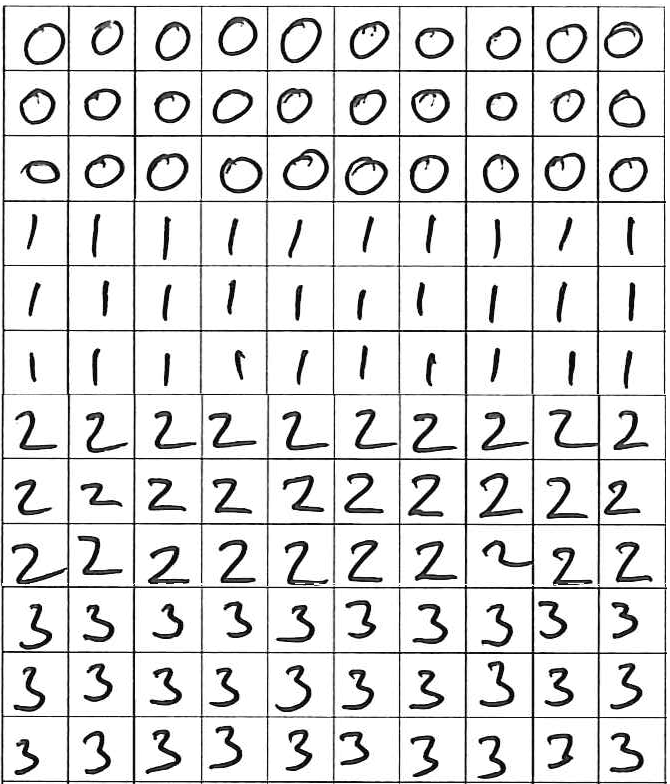
\includegraphics[width=0.7\textwidth]{graphics/digit_example}
\end{center}

\newpage

\tableofcontents
\listoffigures
\listoftables

\newpage


%\section{K-Nearest Neighbours}

% % % Part one
% \subsection{Theory}
The K-Nearest Neighbour (K-NN) method is in this report used to classify a unknown digit to a set of known digits ranging from zero to nine.
%The data is split into two groups: One is for training and one is for testing. 
A set of the $k$ nearest neighbour is found using the euclidean distance to the pixel values in a training set of which the elements are already classified.
The result from the classification is found by counting the number of occurrences from the set of the $k$ nearest neighbours and choosing the most prominent.

%To see how this method performs a multitude of tests are performed to see how multiple parameters affect the success rate and the speed.

An example of such is seen in figure \ref{fig:knn_illustration}.

\begin{figure}[H]
\centering
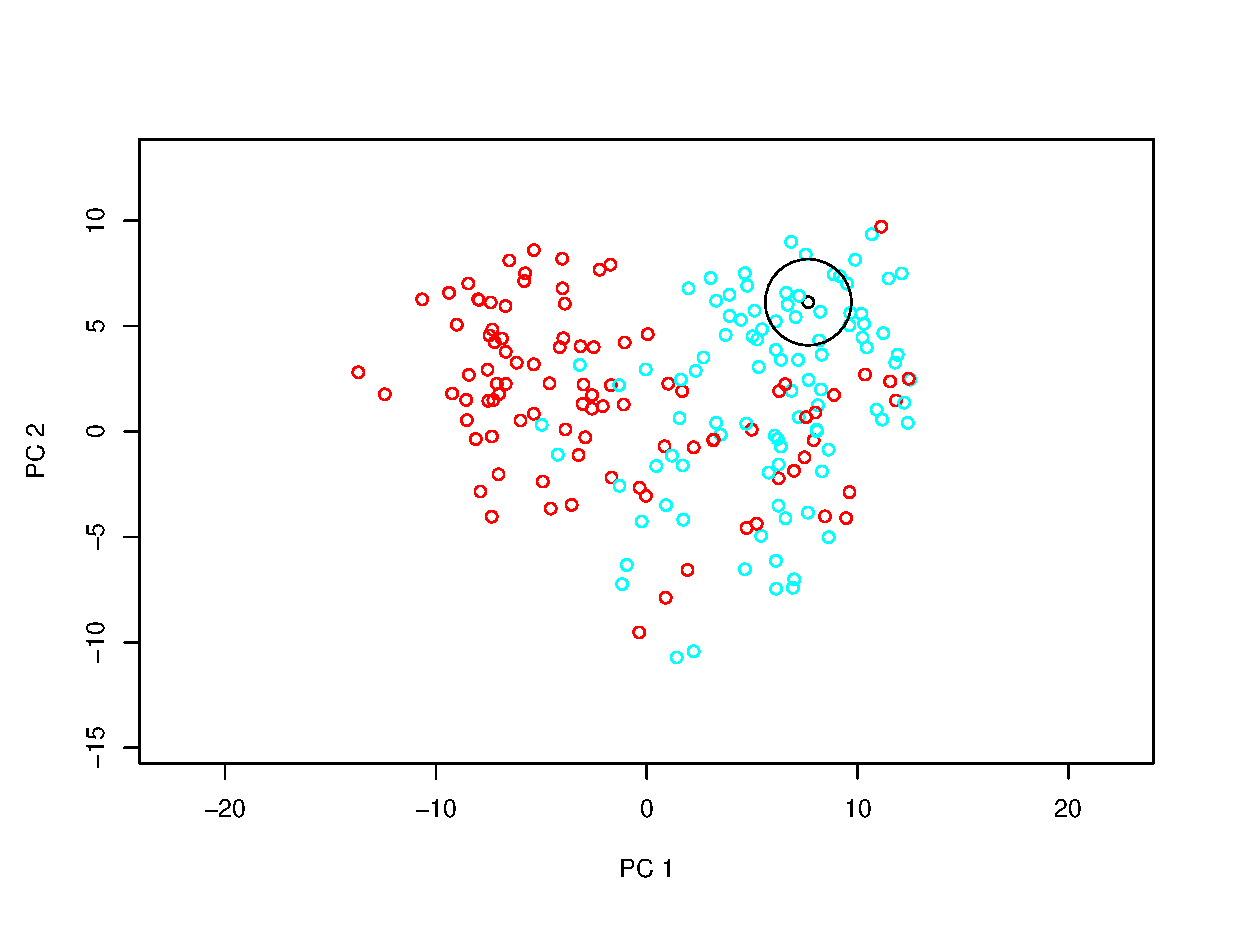
\includegraphics[width = 0.8 \textwidth]{graphics/knn_vis}
\caption[Illustration of the K-NN approach.]{Illustration of the K-NN approach with $k = 10$ on the normalized data for two classes plotting the two most prominent principle components.}
\label{fig:knn_illustration}
\end{figure}

In figure \ref{fig:knn_illustration} the black data point is an element of the blue test set.
The circle around it encircles the ten nearest neighbours.
Since there are more blue neighbours within the circle than red, then the classification in this case correctly classifies the element to the blue one.

\todo[inline]{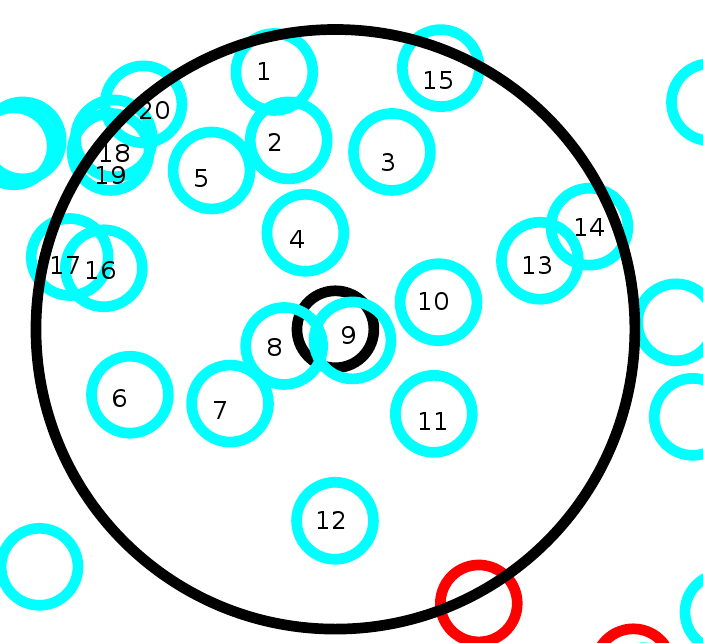
\includegraphics[width=0.2\textwidth]{graphics/knn_circle} Kan vi lave en cirkel om de 10 nærmeste?}

% %\subsection{K-NN Implementation}


\lstinputlisting[language = R,
firstnumber = 291,
firstline = 291, 
lastline = 311, 
captionpos=b,
caption = {K-NN implementation.}]{../Code/KNN/01/test.R}

% %1.5.1
%50/50, k = 10 -> tid vs DPI!
%confusion matrix på 1 run (100, 200 og 300 DPI) 
%1.5.2
%k vs Train Size (10 runs)
%1.5.3
%cross val. 10 runs 90/10 -> mean + var


\subsection{Single Person Tests}
This section tests the K-NN algorithm using data from one single person, namely Group three member two's data.
%
%The tests are performed first with the data split equally into a 50\% for the training and 50\% for the test set and the runtime is measured and compared for the three different image qualities. 
%
%Then test are performed with changing values of k and the training set size.
%
%Afterwards with a 90/10\% split for training and test respectively is computed and mean and variance is given.
%
%All the tests will be conducted using cross validation with 10 runs.

\subsubsection{Equally Sized training and test set}
To test the algorithm the data from the three different DPI's where split 50/50\% into a training and test set. 
The time to compute the test set for each DPI was then recorded and plotted. This is seen in figure \ref{fig:PersonDependent_5050}.
As expected does this scale with number of pixels. 

% % % % generated by timing.R
\begin{figure}[h]
\centering
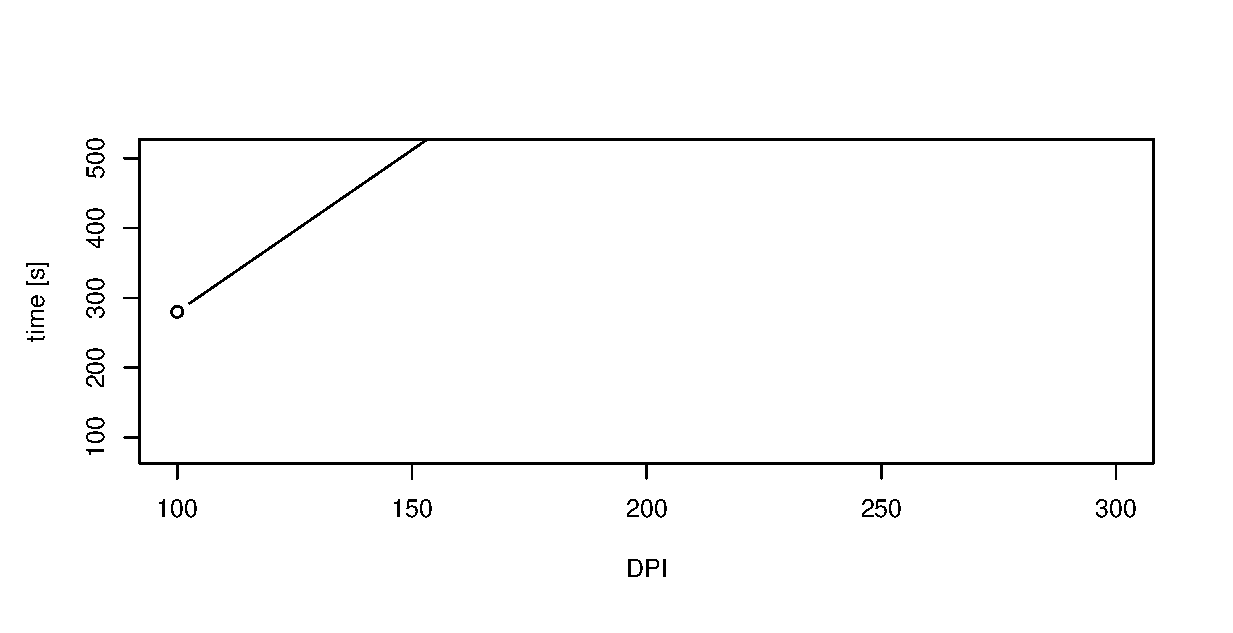
\includegraphics[width=\textwidth]{graphics/time_vs_dpi}
\caption{Timing of running a result with a 50/50\% split of group three member two's data}
\label{fig:PersonDependent_5050}
\end{figure}

Running the three test sets resulted in the confusion matrices seen in table \ref{tb:confus}.
They are all tested with a K of 10 and a split of 50/50\%.
In these it is seen which numbers do well and which numbers are hard to detect and which number they are detected as.
While the chance of matching a 1 with a 1 is really high there seem to be a high chance of getting a false positive as only 200 out of the 440 detected ones actually were correct.
And while the overall detection is good, the 8 is hard to detect with only 57\% success rate on 300 dpi.

% % % % generated by confusion.R
\begin{table}
    \centering
    \begin{subtable}{0.5\textwidth}
        \flushright
        
\begin{tikzpicture}
            \node at (0,0) {};
            \node at (1,0) {\huge Correct number}; 
        \end{tikzpicture}
    \end{subtable}

    \begin{subtable}{0.1\textwidth}
        \flushright
        
\begin{tikzpicture}
            \node[rotate=90] {\huge Guessed number};
        \end{tikzpicture}
    \end{subtable}
    \begin{subtable}{0.6\textwidth}
        \begin{subtable}{\textwidth}
            \centering
            {\scriptsize
                \begin{tabular}{l|*{10}{c}}
                    &0	& 1	& 2	& 3	& 4	& 5	& 6	& 7	& 8	& 9 \\
\hline
0	& 172	& 0	& 0	& 0	& 2	& 2	& 5	& 0	& 0	& 0 \\
1	& 18	& 199	& 24	& 21	& 30	& 26	& 25	& 19	& 32	& 57 \\
2	& 2	& 0	& 147	& 3	& 1	& 3	& 2	& 3	& 4	& 1 \\
3	& 5	& 1	& 14	& 172	& 0	& 6	& 18	& 6	& 34	& 14 \\
4	& 0	& 0	& 0	& 0	& 159	& 4	& 1	& 2	& 1	& 20 \\
5	& 0	& 0	& 0	& 0	& 0	& 154	& 0	& 0	& 2	& 0 \\
6	& 1	& 0	& 0	& 1	& 0	& 1	& 149	& 0	& 1	& 0 \\
7	& 0	& 0	& 10	& 2	& 0	& 0	& 0	& 169	& 0	& 1 \\
8	& 0	& 0	& 4	& 0	& 0	& 4	& 0	& 1	& 106	& 5 \\
9	& 2	& 0	& 1	& 1	& 8	& 0	& 0	& 0	& 20	& 102 \\

                \end{tabular}
            }
            \caption{Results for 100 DPI}
        \end{subtable}
        \begin{subtable}{\textwidth}
            \centering
            {\scriptsize
                \begin{tabular}{l|*{10}{c}}
                    &0	& 1	& 2	& 3	& 4	& 5	& 6	& 7	& 8	& 9 \\
\hline
0	& 172	& 0	& 0	& 0	& 1	& 3	& 0	& 0	& 1	& 1 \\
1	& 26	& 200	& 18	& 37	& 23	& 11	& 24	& 16	& 39	& 58 \\
2	& 0	& 0	& 160	& 2	& 0	& 1	& 4	& 0	& 2	& 0 \\
3	& 0	& 0	& 7	& 155	& 0	& 1	& 20	& 1	& 20	& 16 \\
4	& 0	& 0	& 0	& 0	& 168	& 1	& 0	& 1	& 0	& 6 \\
5	& 0	& 0	& 0	& 0	& 0	& 181	& 1	& 0	& 1	& 0 \\
6	& 2	& 0	& 0	& 0	& 1	& 0	& 150	& 0	& 4	& 0 \\
7	& 0	& 0	& 13	& 5	& 0	& 0	& 1	& 182	& 1	& 2 \\
8	& 0	& 0	& 1	& 0	& 0	& 1	& 0	& 0	& 103	& 1 \\
9	& 0	& 0	& 1	& 1	& 7	& 1	& 0	& 0	& 29	& 116 \\

                \end{tabular}
            }
            \caption{Results for 200 DPI}
        \end{subtable}
        \begin{subtable}{\textwidth}
            \centering
            {\scriptsize
                \begin{tabular}{l|*{10}{c}}
                    &0	& 1	& 2	& 3	& 4	& 5	& 6	& 7	& 8	& 9 \\
\hline
0	& 157	& 0	& 0	& 0	& 1	& 4	& 2	& 0	& 0	& 0 \\
1	& 37	& 200	& 24	& 33	& 17	& 14	& 18	& 19	& 30	& 48 \\
2	& 1	& 0	& 160	& 0	& 0	& 0	& 2	& 0	& 2	& 0 \\
3	& 1	& 0	& 1	& 152	& 0	& 0	& 7	& 1	& 15	& 9 \\
4	& 0	& 0	& 0	& 0	& 179	& 0	& 0	& 0	& 2	& 5 \\
5	& 0	& 0	& 0	& 0	& 1	& 181	& 0	& 0	& 1	& 0 \\
6	& 4	& 0	& 0	& 0	& 1	& 0	& 162	& 0	& 2	& 0 \\
7	& 0	& 0	& 15	& 15	& 0	& 0	& 9	& 180	& 3	& 2 \\
8	& 0	& 0	& 0	& 0	& 0	& 1	& 0	& 0	& 114	& 0 \\
9	& 0	& 0	& 0	& 0	& 1	& 0	& 0	& 0	& 31	& 136 \\

                \end{tabular}
            }
            \caption{Results for 300 DPI}
        \end{subtable}
    \end{subtable}
    \caption{Confusion matrices with different scaling}
    \label{tb:confus}
\end{table}

\subsubsection{Changing K and Training Set Size}
Tests was performed to see how both the value of K and size of the training set affects the accuracy of the K-NN algorithm. 
The result is given in figure \ref{fig:personDependent_contour}.

% \begin{figure}[H]
% \centering
% 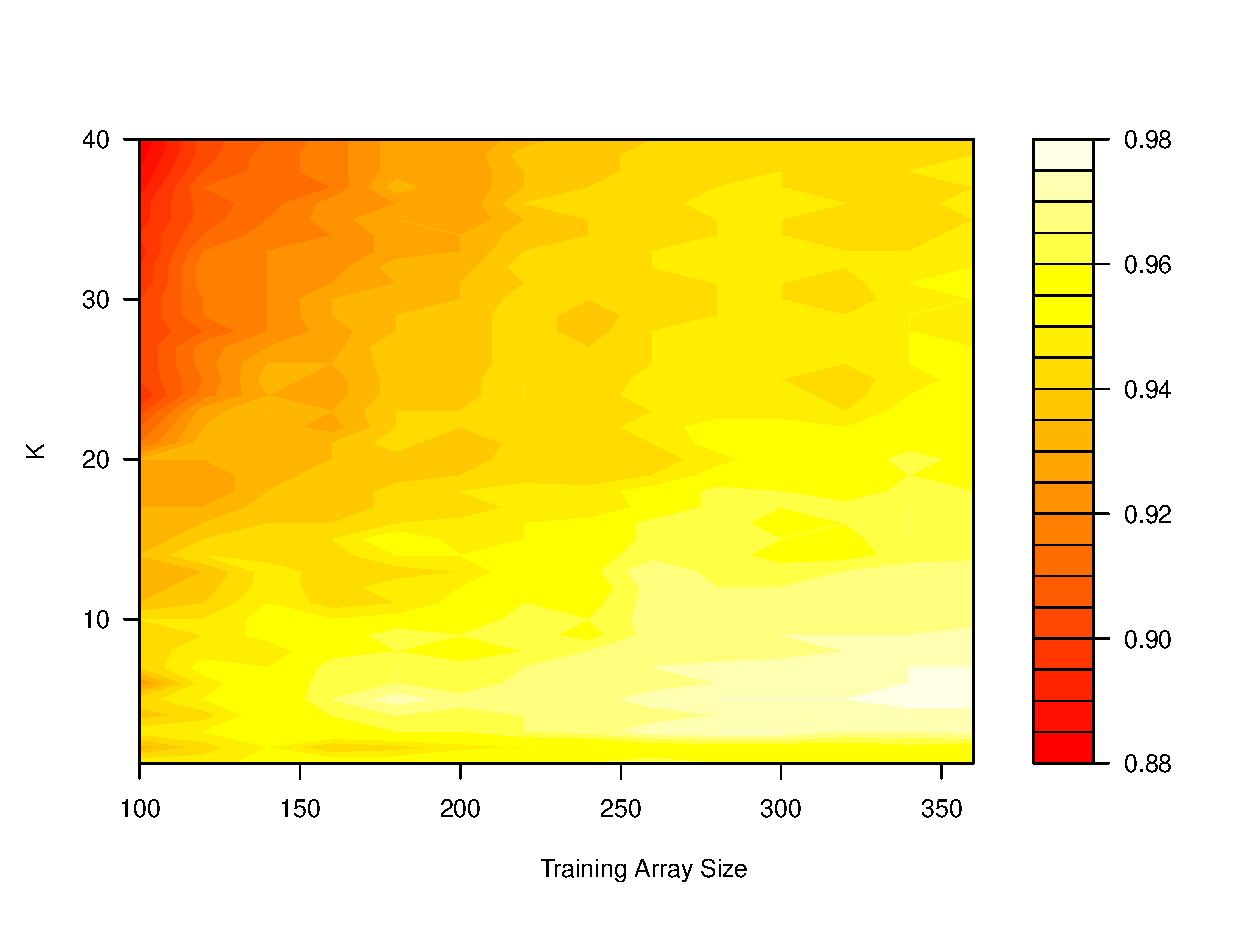
\includegraphics[width = 13cm]{graphics/graph_G3M2_20}
% \caption{Success Rate of the K-NN algorithm for changing values of K and the training set size.}
% \label{fig:personDependent_contour}
% \end{figure}

\begin{figure}[H]
\centering
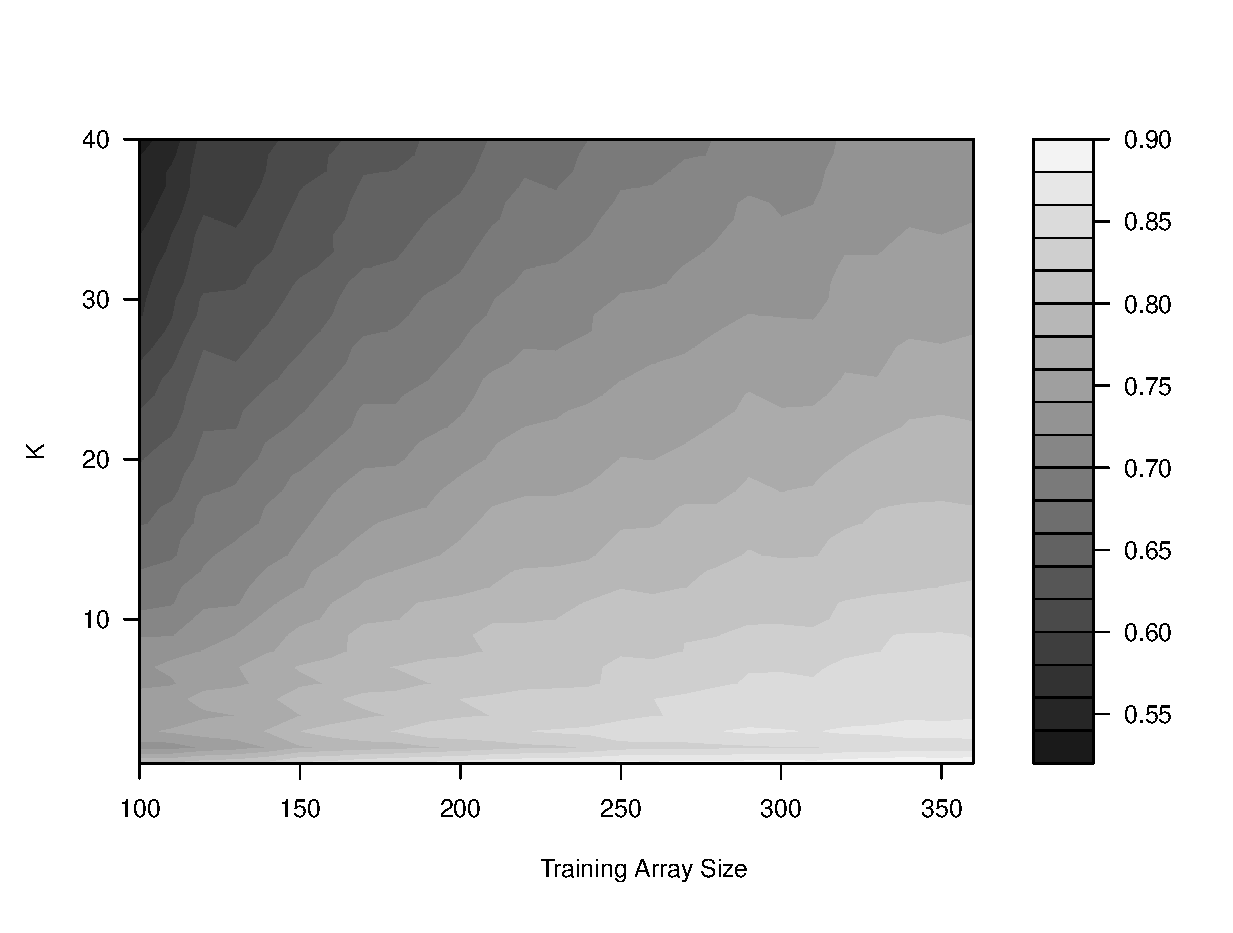
\includegraphics[width = 13cm]{graphics/graph_G3M2_10_10}
\caption{Success Rate of the K-NN algorithm for changing values of K and the training set size.}
\label{fig:personDependent_contour}
\end{figure}

% \begin{figure}[H]
% \centering
% 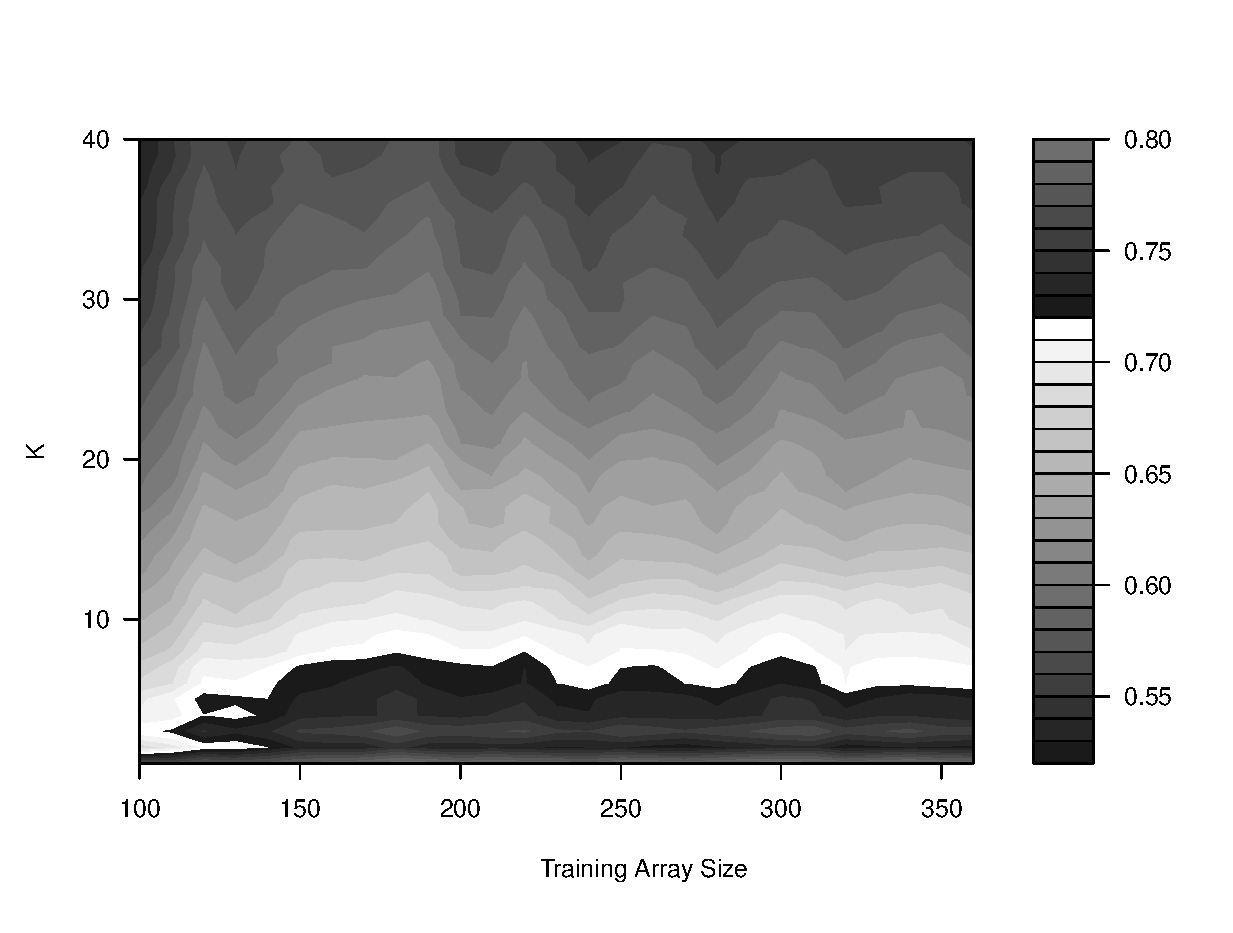
\includegraphics[width = 13cm]{graphics/graph_G3M1_10_10}
% \caption{Success Rate of the K-NN algorithm for changing values of K and the training set size.}
% \label{fig:personDependent_contour}
% \end{figure}

The test conducted in figure \ref{fig:personDependent_contour} where done with a test size of 40 and run 10 times with cross validation.

As seen on figure \ref{fig:personDependent_contour}, then the accuracy of the algorithm appears to increase as the train set size increases.
Furthermore the optimal value of K is dependent on the size of training set. 
As the size of the training set increases, so does the area where a the best performance is obtained.
From figure \ref{fig:personDependent_contour} it can be seen that the results are best when using a training size which is above 300 and K ranging between 3 and 7.


\subsubsection{90/10 Data Split}
A cross validation was also carried out using a 90/10\% and 50/50\% split of the data. 
Each test was made on both group members to see the difference.
The result of this is seen in figure \ref{fig:PersonDependent_9010}.
The values can be seen in \ref{tb:cross}

% % % % Generating this with cross_test.R tonight
\begin{figure}[h]
\centering
% 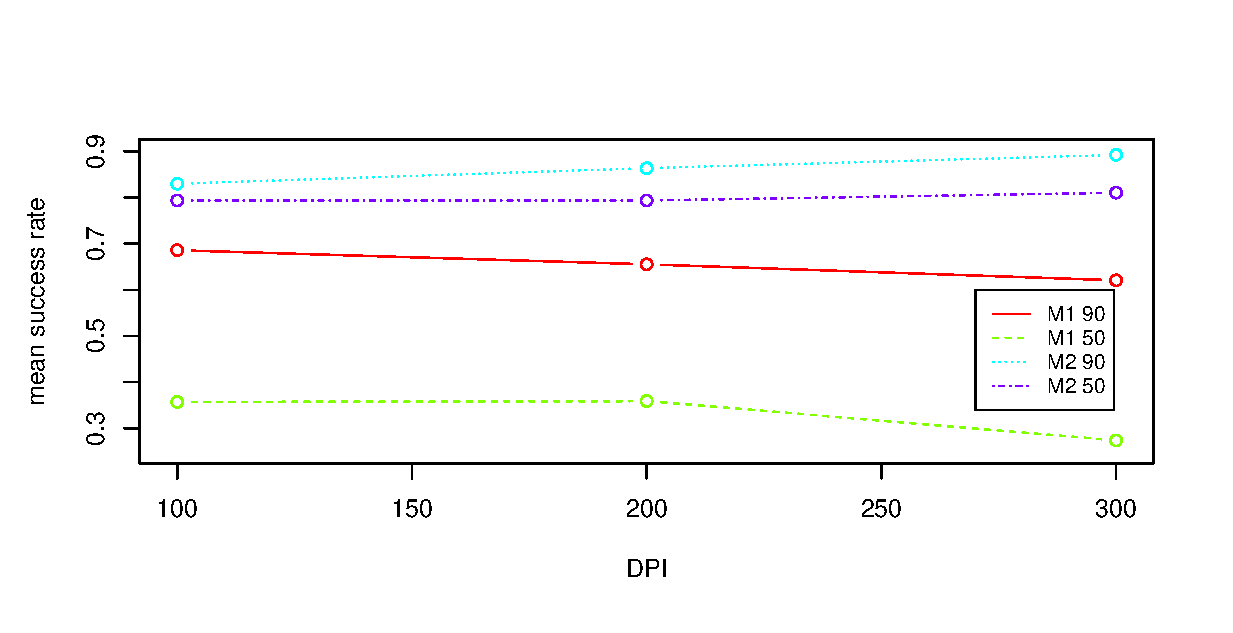
\includegraphics[width=\textwidth]{graphics/cross_test}
\caption[Cross validation]{Test result with a 90/10\% and 50/50\% split. The data points are taken as the mean of 10 runs using cross validation.}
\label{fig:PersonDependent_9010}
\end{figure}

\begin{table}[h]
\centering
    \begin{subtable}[b]{0.56\textwidth}
    \centering
        \begin{tabular}{lcccccc}
%             &M1 90	& M1 50	& M2 90	& M2 50 \\
\hline
100	& 0.6857	& 0.3570	& 0.8297	& 0.7935 \\
200	& 0.6552	& 0.3590	& 0.8635	& 0.7935 \\
300	& 0.6205	& 0.2735	& 0.8925	& 0.8105 \\

        \end{tabular}
        \caption{Mean success rate}
    \end{subtable}
    \begin{subtable}[b]{0.42\textwidth}
    \centering
        \begin{tabular}{lcccccc}
%             &M1 90	& M1 50	& M2 90	& M2 50 \\
\hline
100	& 0.0261	& 0.0253	& 0.01193	& 0.0223 \\
200	& 0.0275	& 0.8602	& 0.01100	& 0.0223 \\
300	& 0.0399	& 0.0708	& 0.00552	& 0.0154 \\

        \end{tabular}
        \caption{Variance in success rate}
    \end{subtable}
    \caption[Success of functions]{Success mean and variance of different split and data sets.}
    \label{tb:cross}
\end{table}





% % 1.6.2: tabel over mean+var over 10 runs + 
%        graf dpi vs success for filtre (10 run)

\subsection{Preprocessed Image - Single Person Tests}

\begin{table}[h]
\centering
    \begin{subtable}[b]{0.56\textwidth}
    \centering
        \begin{tabular}{lcccccc}
            &Raw	& Avg	& G 0.5	& G 1	& G 2 \\
\hline
100	& 0.8297	& 0.860	& 0.8297	& 0.8545	& 0.7750 \\
200	& 0.8635	& 0.895	& 0.8635	& 0.8998	& 0.8602 \\
300	& 0.8925	& 0.920	& 0.8925	& 0.9190	& 0.8842 \\

        \end{tabular}
        \caption{Mean success rate.}
    \end{subtable}
    \begin{subtable}[b]{0.42\textwidth}
    \centering
        \begin{tabular}{lcccccc}
            &Raw	& Avg	& G 1	& G 2	& G 3 \\
\hline
100	& NA	& NA	& NA	& NA	& NA \\
200	& NA	& NA	& NA	& NA	& NA \\
300	& NA	& NA	& NA	& NA	& NA \\

        \end{tabular}
        \caption{Variance in success rate.}
    \end{subtable}
    \caption[Success of smoothing functions.]{Mean success rate and variance of different smoothing functions.}
    \label{tb:smooth}
\end{table}

\begin{figure}[h]
\centering
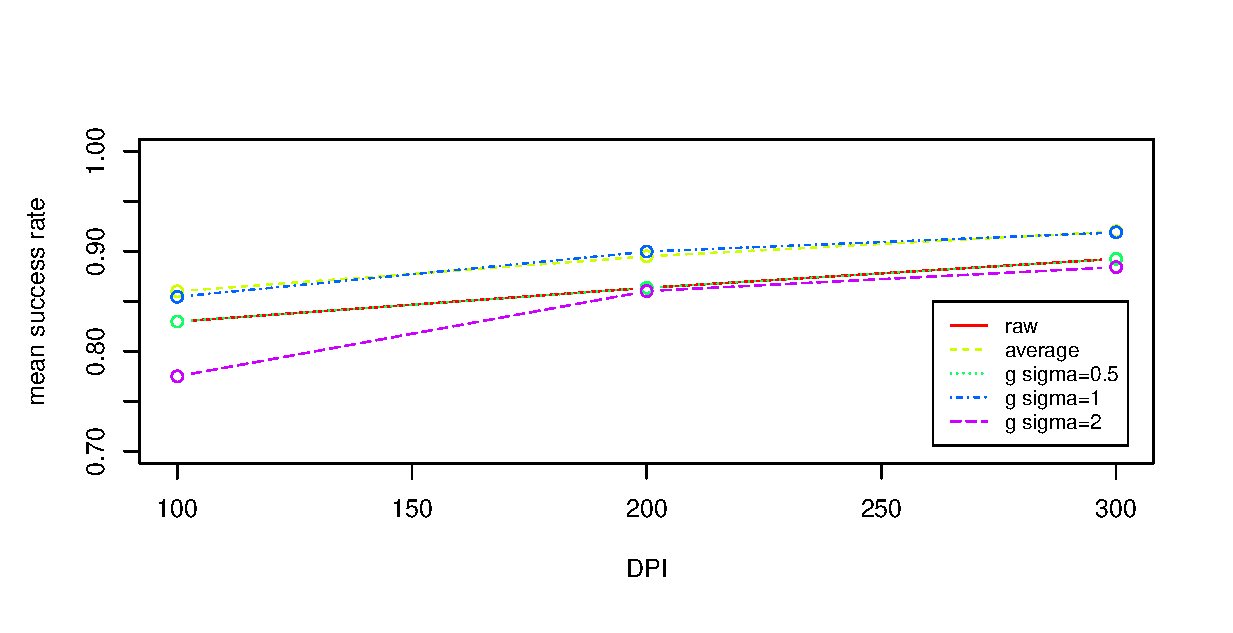
\includegraphics[width=1\textwidth]{graphics/smoothing}
\caption{Success rate of smoothing functions.}
\label{fig:smooth}
\end{figure}

Applying a smoothing function can give the image an advantage when using the nearest neighbour analysis.
By taking an average of the neighbouring pixels the lines in the digit should be wider and the digits should have a better chance of overlapping.
The danger is that too much smoothing could make the whole image one colour and would completely destroy any chance of analysis.
A Gaussian distribution (also referred to as a normal distribution) a naturally occurring distribution that happens when a random result occurs around a mean. 
The $\sigma$ signifies the deviation of the distribution. 
The 2D equation of a Gaussian distribution is shown in equation \ref{eq:gauss}. 

\begin{equation}
G(x,y) = \frac{1}{2\pi \sigma^2} e^{- \frac{x^2+y^2}{2\sigma^2}} \label{eq:gauss}
\end{equation}

Using the Gaussian filter to smooth an image will weigh the distance to the pixel.
A small $\sigma$ will make a small deviation and thus heavily weigh the center pixel.
The results of the filtering methods were also compared to the raw image with 100, 200 and 300 DPI.
These results are compared with an averaging filter (avg) which takes the average of the four neighbouring pixels and a Gaussian filter (G) with different values for sigma.
These tests were done 10 times, using cross validation, and the mean of each success rate is plotted in figure \ref{fig:smooth}. 
Since the variance is too small to be seen in the figure the mean and variance is shown in table \ref{tb:smooth}.
The averaging filter does not give a measurable different result from not using a filter.
The Gaussian filter does improves the success rate for some values of sigma, but a larger $\sigma$ makes it worse.


\section{K-NN on Big Data}
% \section{Introduction}
The classification of handwritten characters is used in a wide range of products to day.
Hence, this report goes in depth with how the numbers from zero to nine can be classified using machine learning algorithms.

The dataset consists of a set of handwritten characters from zero to nine.
These were constructed by the students enrolled in the course Statistical Machine learning (RM-SML-E1) of the year 2015 at the University of Southern Denmark (SDU).
The set used in this report is the 100DPI dataset.
Each number is hence stored as a $20px \times 20px$ matrix containing the handwritten character.

The methods used for classification are K-Nearest Neighbours and Decision Trees and Random Forests.
Furthermore a set of different ways to pre-process the data is explored.
Finally the two methods are compared with each at the best parameters and preprocessing settings.



 %not added to git
% % Part two
\subsection{K-NN on Big Data}

\subsection{Principle Component Analysis}
A Principle Component Analysis (PCA) aims at reducing the number of dimension used to represent the features of the data.
This is done by finding the eigenvectors and eigenvalues to the training set and removing some of the components representing the least variance in the data set.
Thus efficiently reducing the dimensions, but still keeping the most significant knowledge about the features.

\begin{figure}[h]
\begin{subfigure}{0.49\textwidth}
\centering
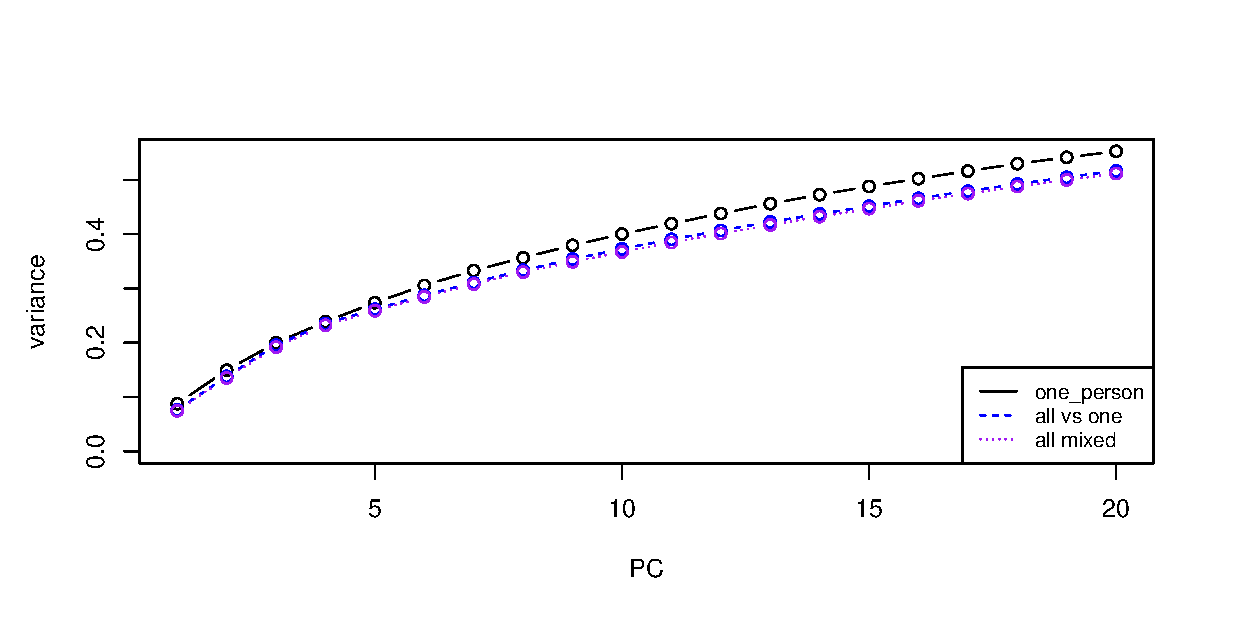
\includegraphics[width=\textwidth]{graphics/pca_acc_variance}
\caption{Accumulated variance}
\label{fig:pca_accumulated_var}
%
\end{subfigure}
\begin{subfigure}{0.49\textwidth}
\centering
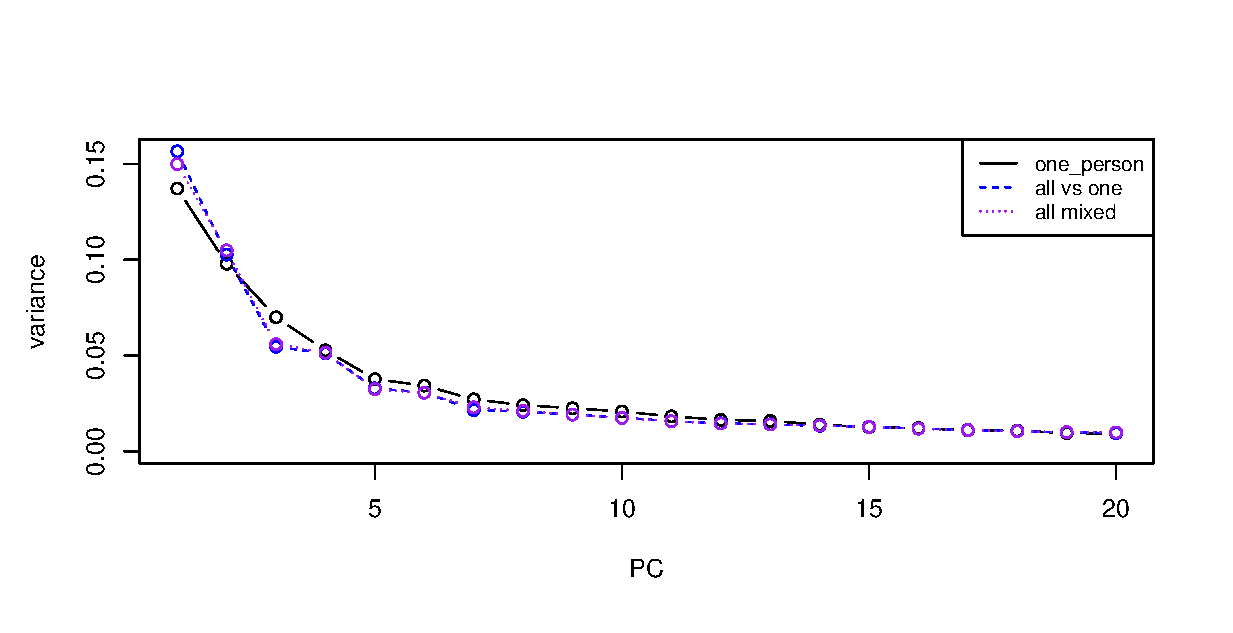
\includegraphics[width=\textwidth]{graphics/pca_variance}
\caption{Variance}
\label{fig:pca_accumulated_var}
\end{subfigure}
\caption[PCA variance]{Variance over the first 20 principle components.
The data was run on Group 3 member 1's data on 100 DPI. }
\label{fig:variance}
\end{figure}
% Figure \ref{fig:contour_KvsPCA_G3M2vsRest} shows a contour plot of how well Group 3 Member 2's  handwriting was predicted successfully for $K$ and the total variance represented of the PC's varying between one and 20 and 0.5 and 1 respectively.

The principle components analysis (PCA) is an tool that can be used to describe the variance in a data set.

By selecting the most significant principle components (PC) the data set can be systematically reduced with minimal changes to performance.
In figure \ref{fig:variance} is the variance and accumulated variance shown for the first 20 PC. 
It is seen that the first PC is the most significant and the variance converges towards zero with more PC.

Calculating with less data will result in a faster computation time. But it can be hard to predict if the performance becomes better or worse.
Choosing too few PC and there is no features left to compare.
To see how the performance and the timing scales both are shown in figure \ref{fig:pca_timing}. K was chosen to be 10.
The success rate has a peak with a low set of attributes so there must be some confusion that gets sorted out. 

\begin{figure}[h]
\centering
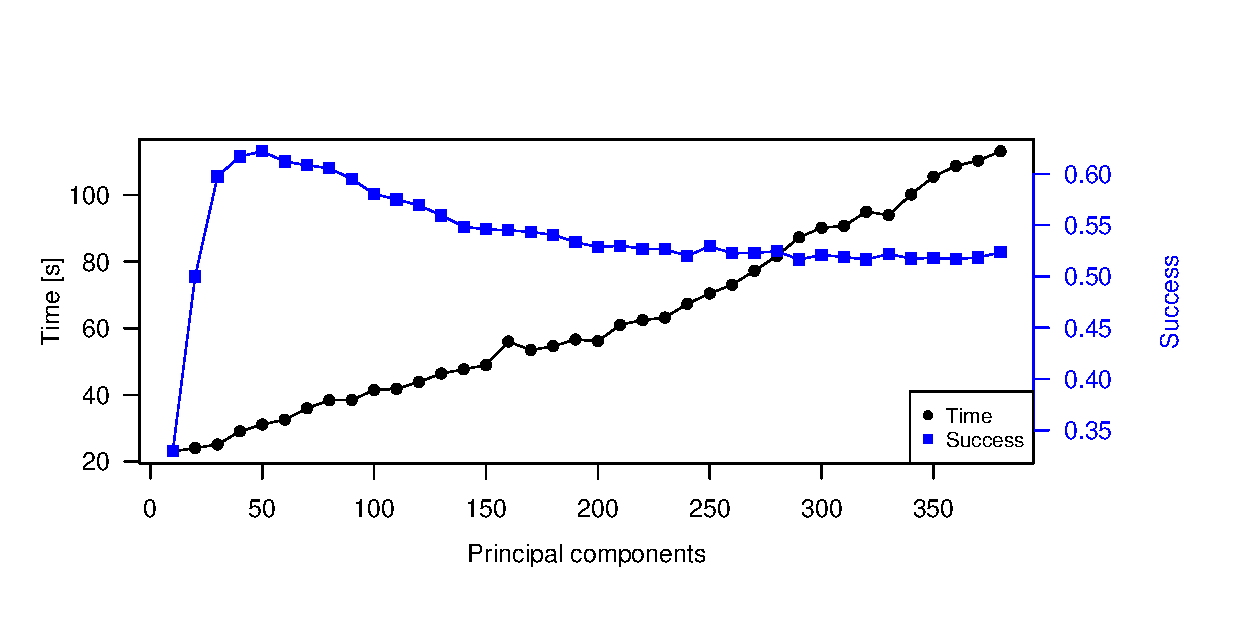
\includegraphics[width =0.8 \textwidth]{graphics/pca_timing_nikolaj}
\caption[Timing of PCA]{Timing of running the PCA with different principle components. 
The data was run on Group 3 member 1's data on 100 DPI. 
The percentage of successful predictions is also measured with the same data.}
\label{fig:pca_timing}
\end{figure}

As seen on figure \ref{fig:contour_KvsPCA_G3M2vsRest}, then the optimum K and represented PCA variance is at $K = 19$ and $PCA = 0.8$. 
This is because an as high successful prediction rate is wanted, but also an as small dataset as possible. 
This point will further be used in section \ref{sec:DataNormalization}.

To get a closer look at how the PCA performs the data from G3M2 was tested against the rest of the class. 
The K was chosen to be 10. 
The data is shown in figure \ref{fig:pca_success}.
The performance is getting worse as more features are considered.

\begin{figure}[h]
\centering
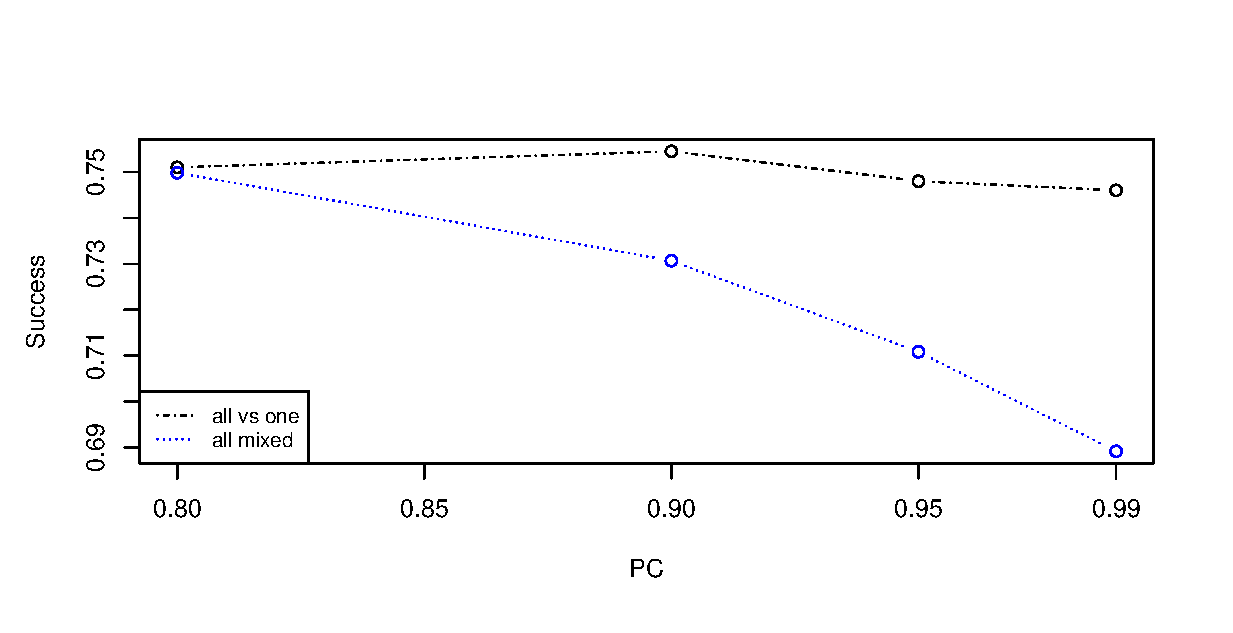
\includegraphics[width =0.8 \textwidth]{graphics/pca_success}
\caption[PCA performance]{Percentage of successful predictions with an increasing accumulated variance used.
The data was run on Group 3 member 2's vs data from 14 members on 100 DPI. }
\label{fig:pca_success}
\end{figure}

To investigate the impact of K the test was redone so more K's were tested and that would lead to finding an optimum K for the large data set.
The data is shown in figure \ref{fig:k_v_PCA}. 
Where the optimum K was very small when testing a single person, a larger K is better suited for tests involving large data sets.
there still seems to be an optimum data size where the full data set performs worse than a smaller data set. 

\begin{figure}[h]
\centering
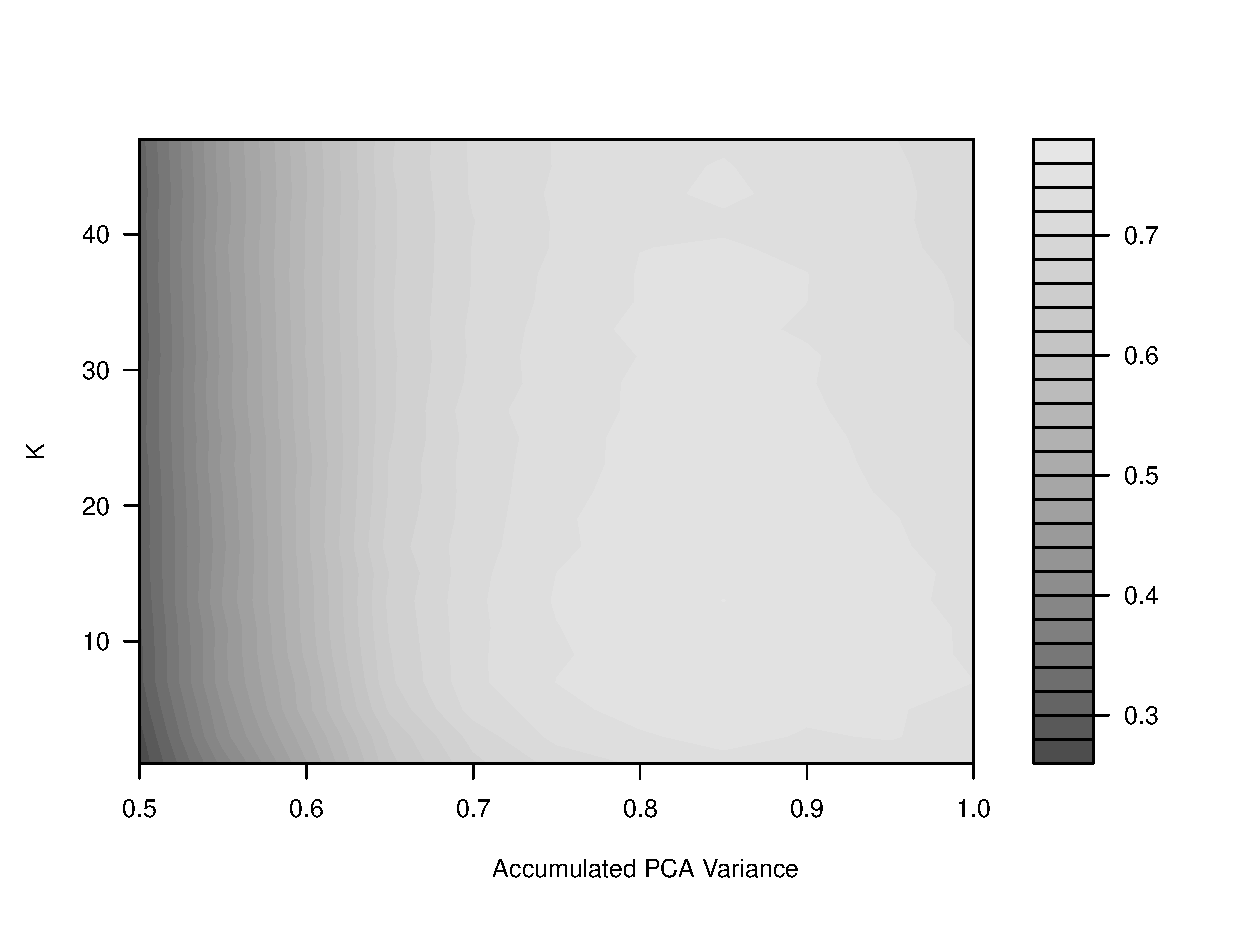
\includegraphics[width = \textwidth]{graphics/contour_k_PCA_oneVsRest}
\caption[Detailed PCA performance]{Success rate for detection of characters of Group 3 Member 2's data when he himself is not represented in the training set. 
The test was done with 16 people.}
\label{fig:k_v_PCA}
\end{figure}




\subsection{Data Normalization and Binning}

\begin{figure}[h]
\centering
    \begin{subfigure}{0.2\textwidth}
        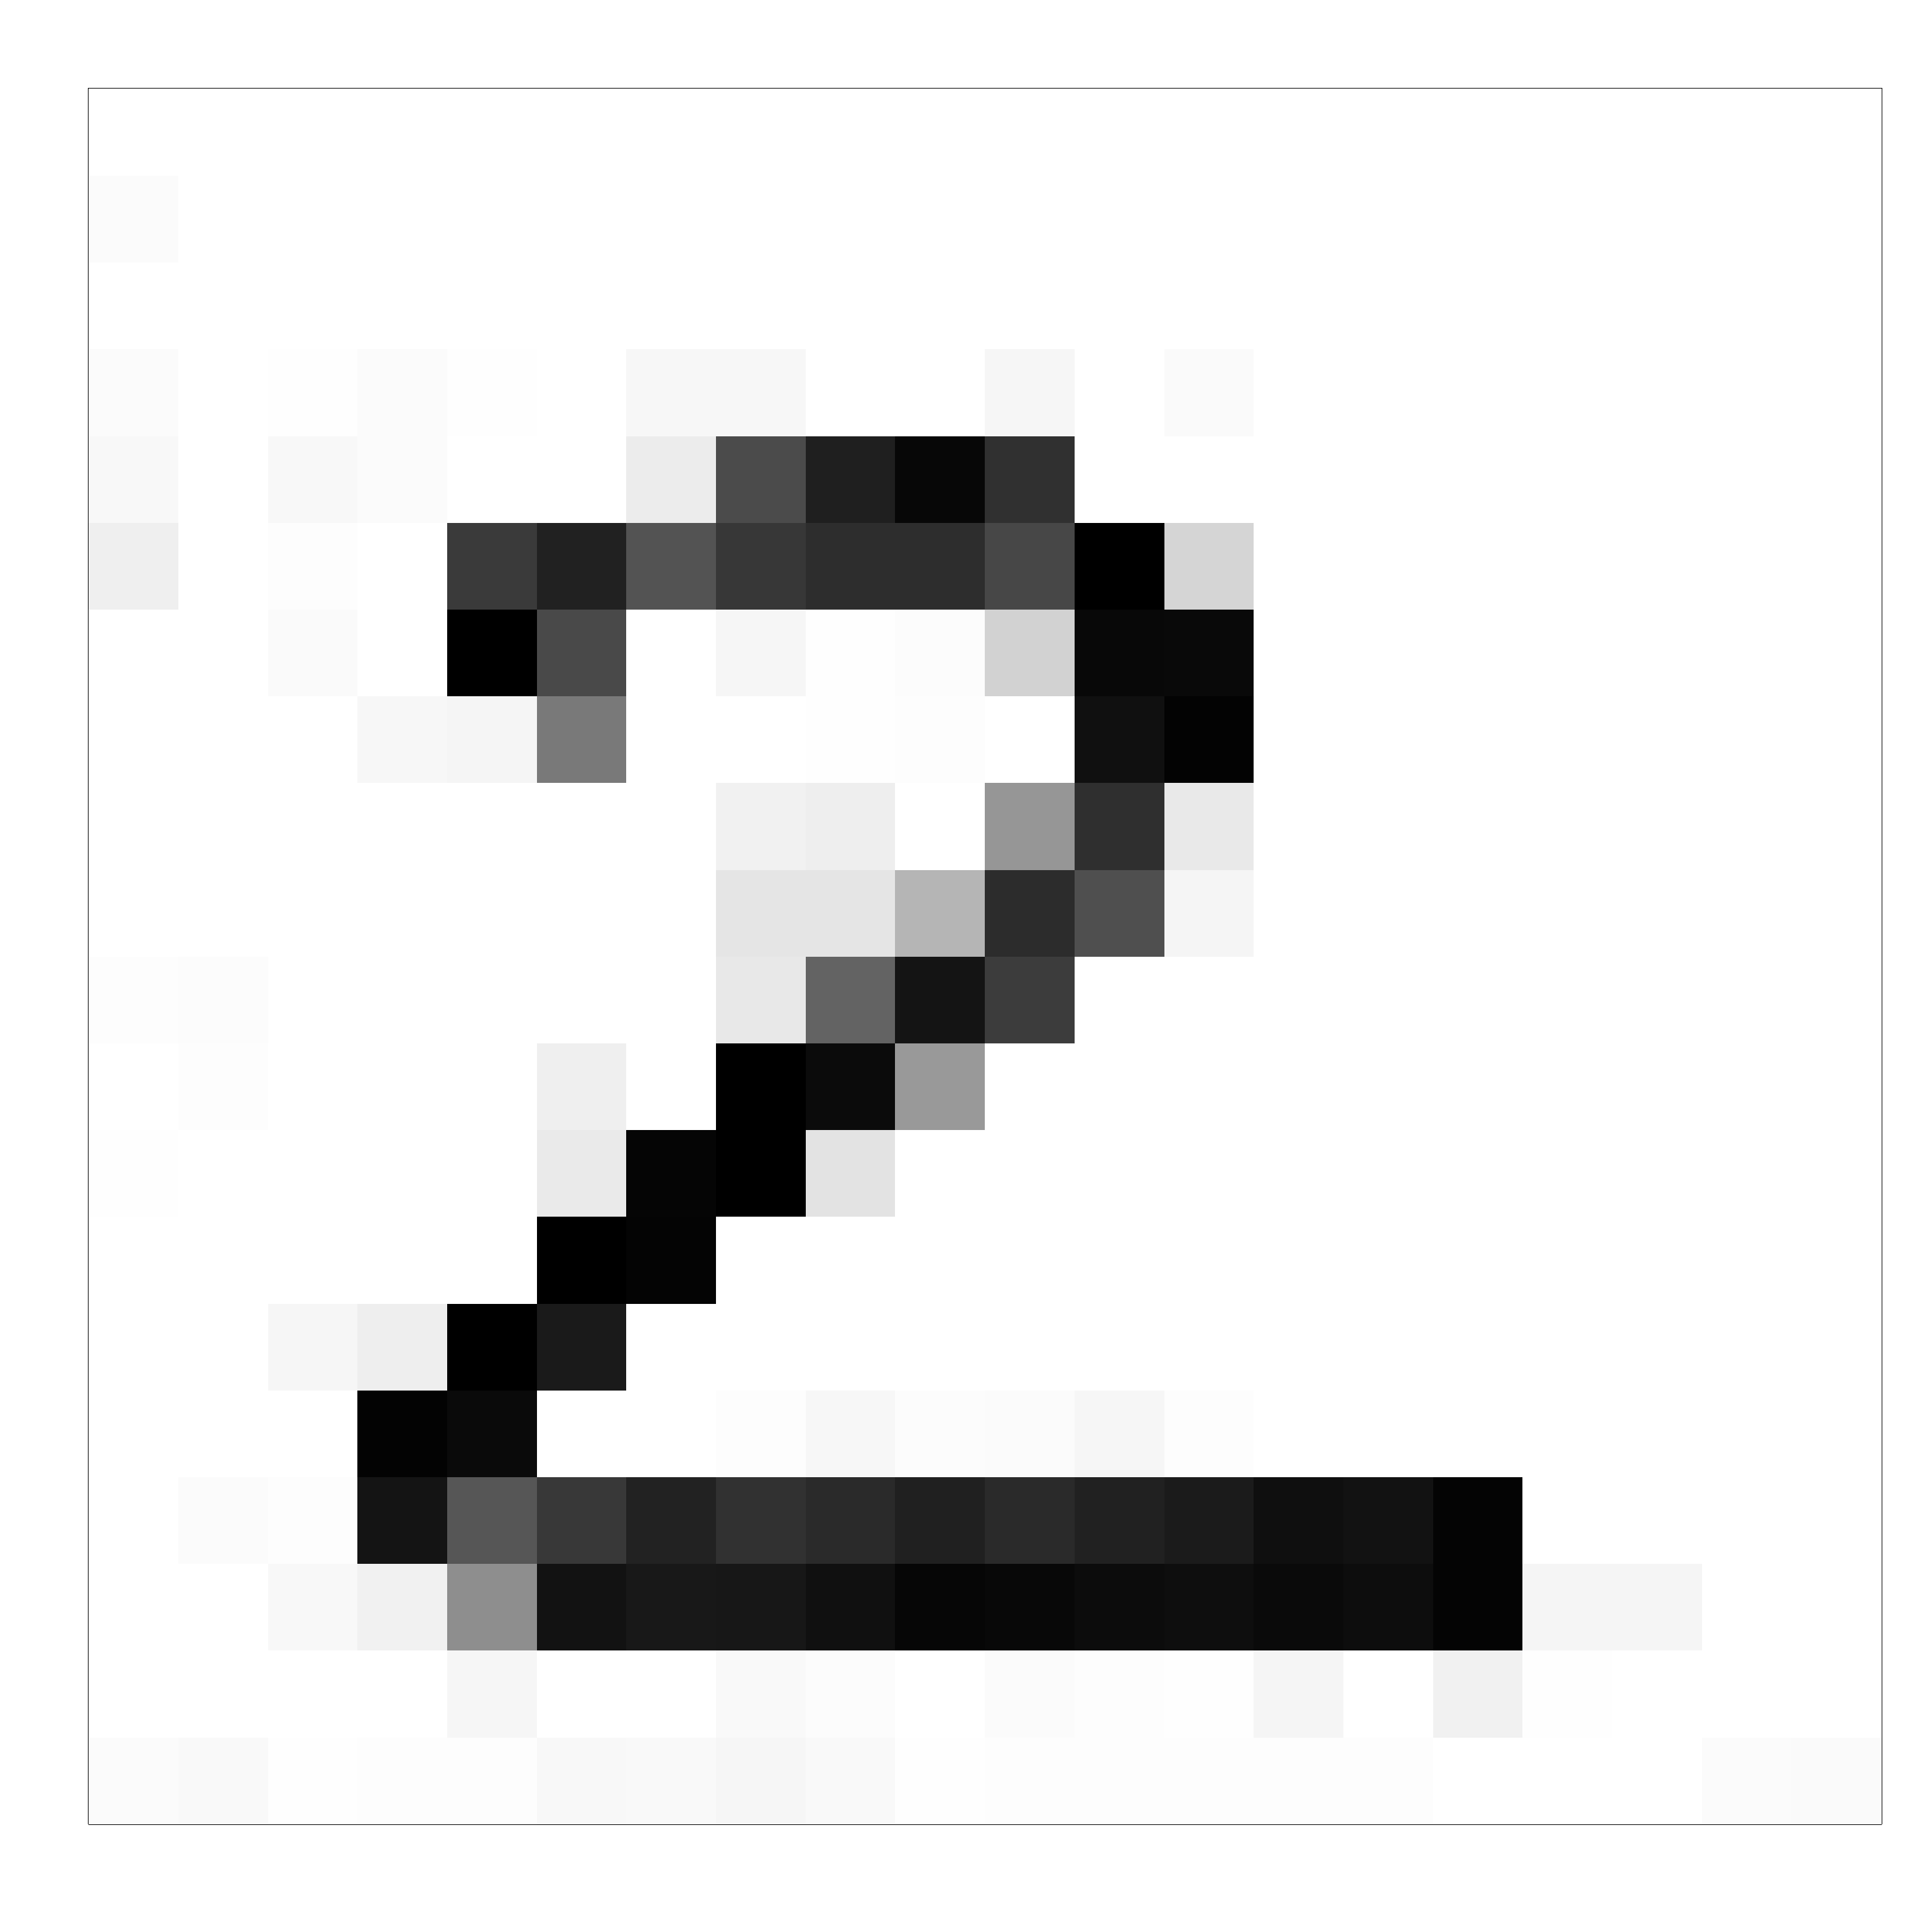
\includegraphics[width = \textwidth]{graphics/bins_inf}
    \end{subfigure}
    \begin{subfigure}{0.2\textwidth}
        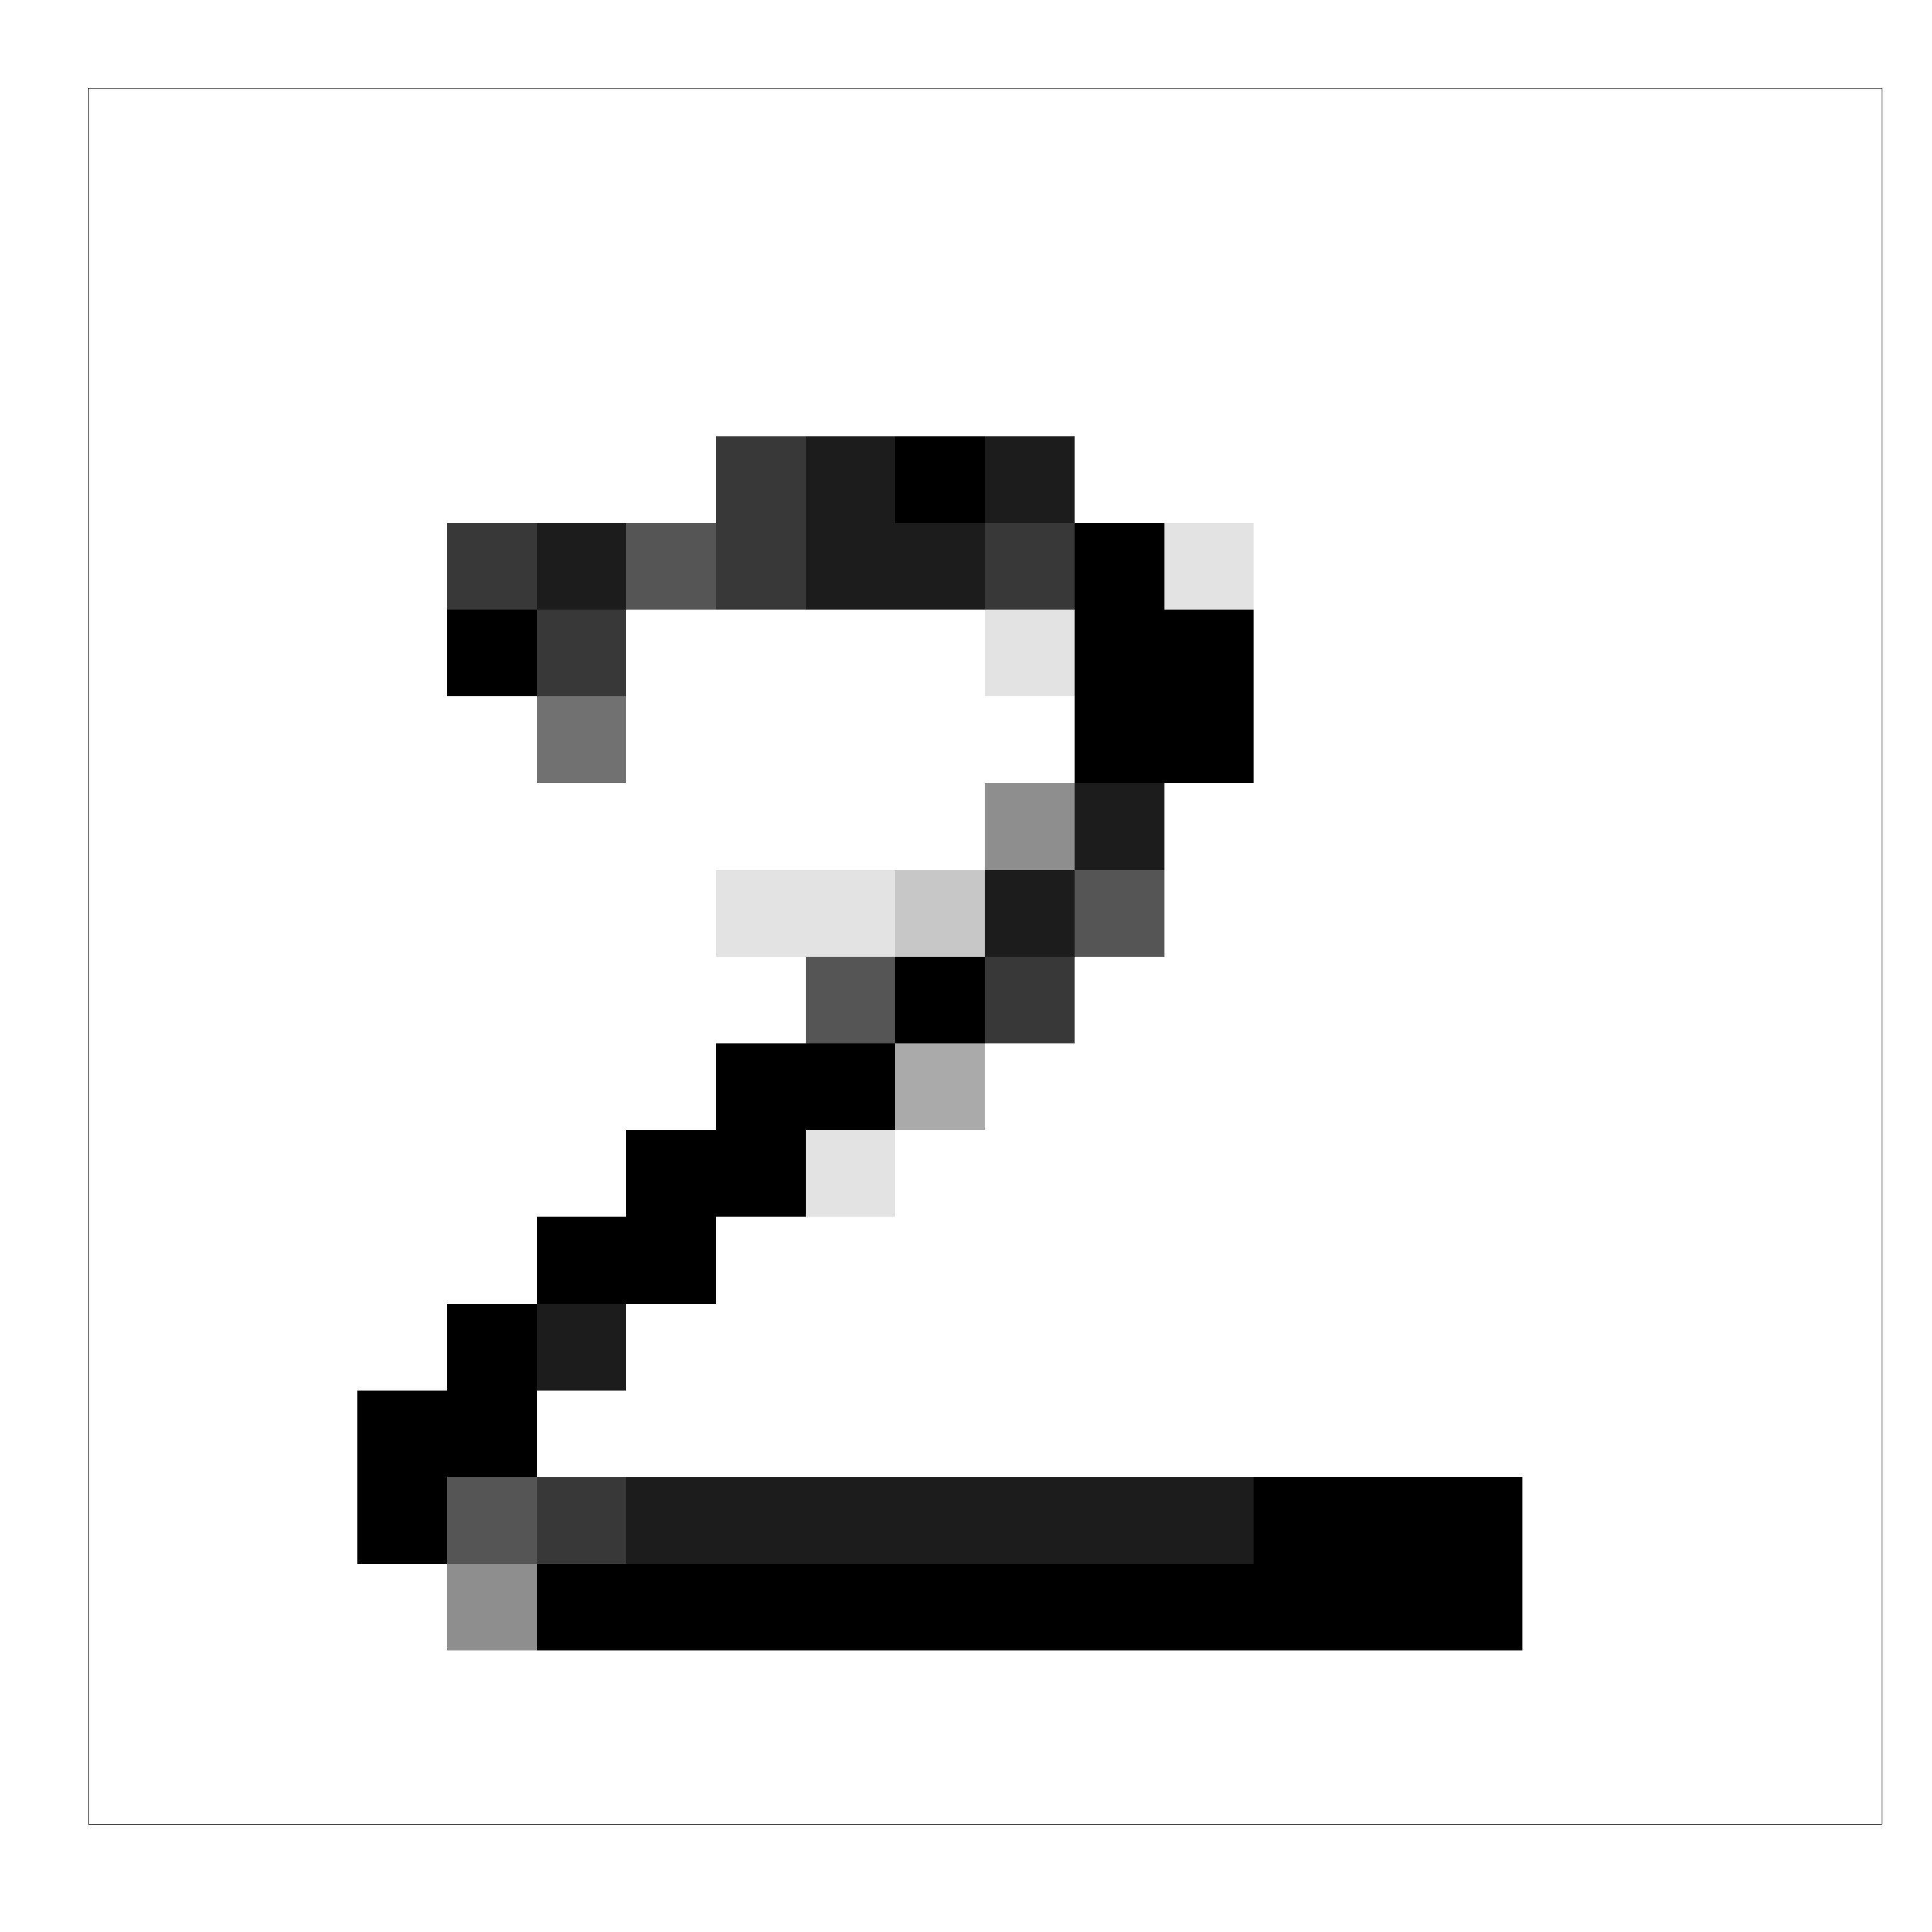
\includegraphics[width = \textwidth]{graphics/bins_10}
    \end{subfigure}
    \begin{subfigure}{0.2\textwidth}
        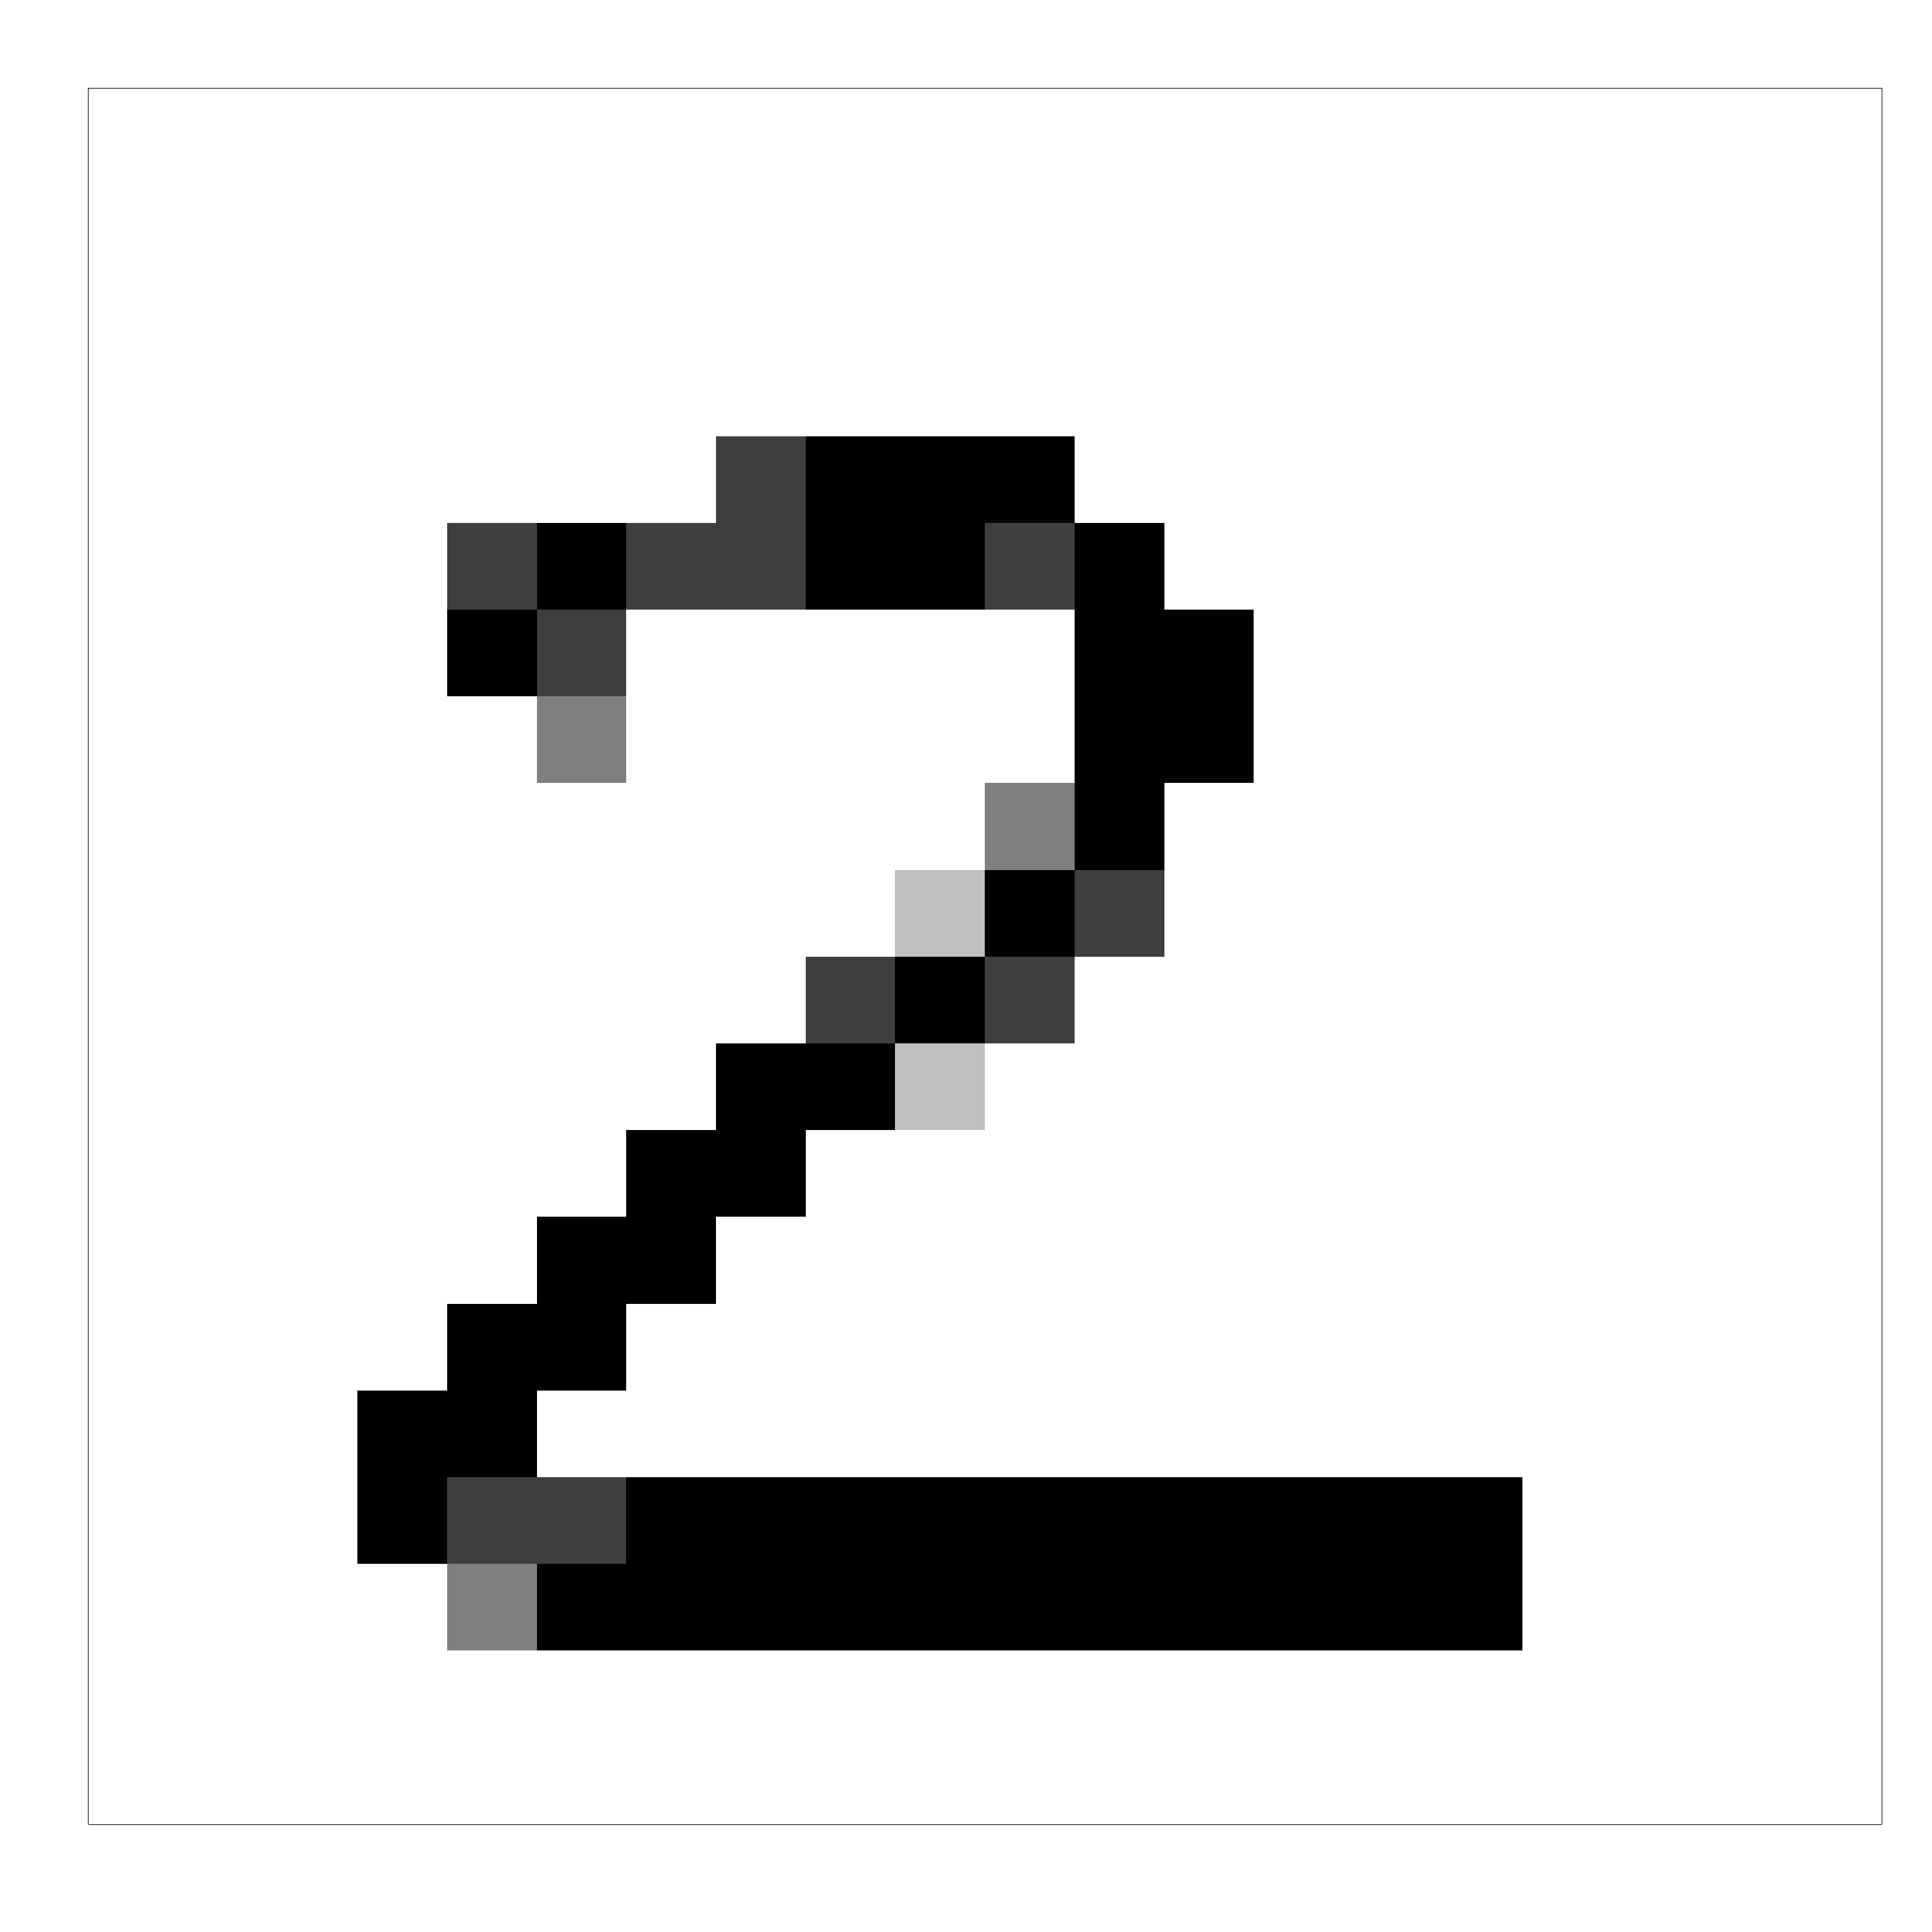
\includegraphics[width = \textwidth]{graphics/bins_5}
    \end{subfigure}
    \begin{subfigure}{0.2\textwidth}
        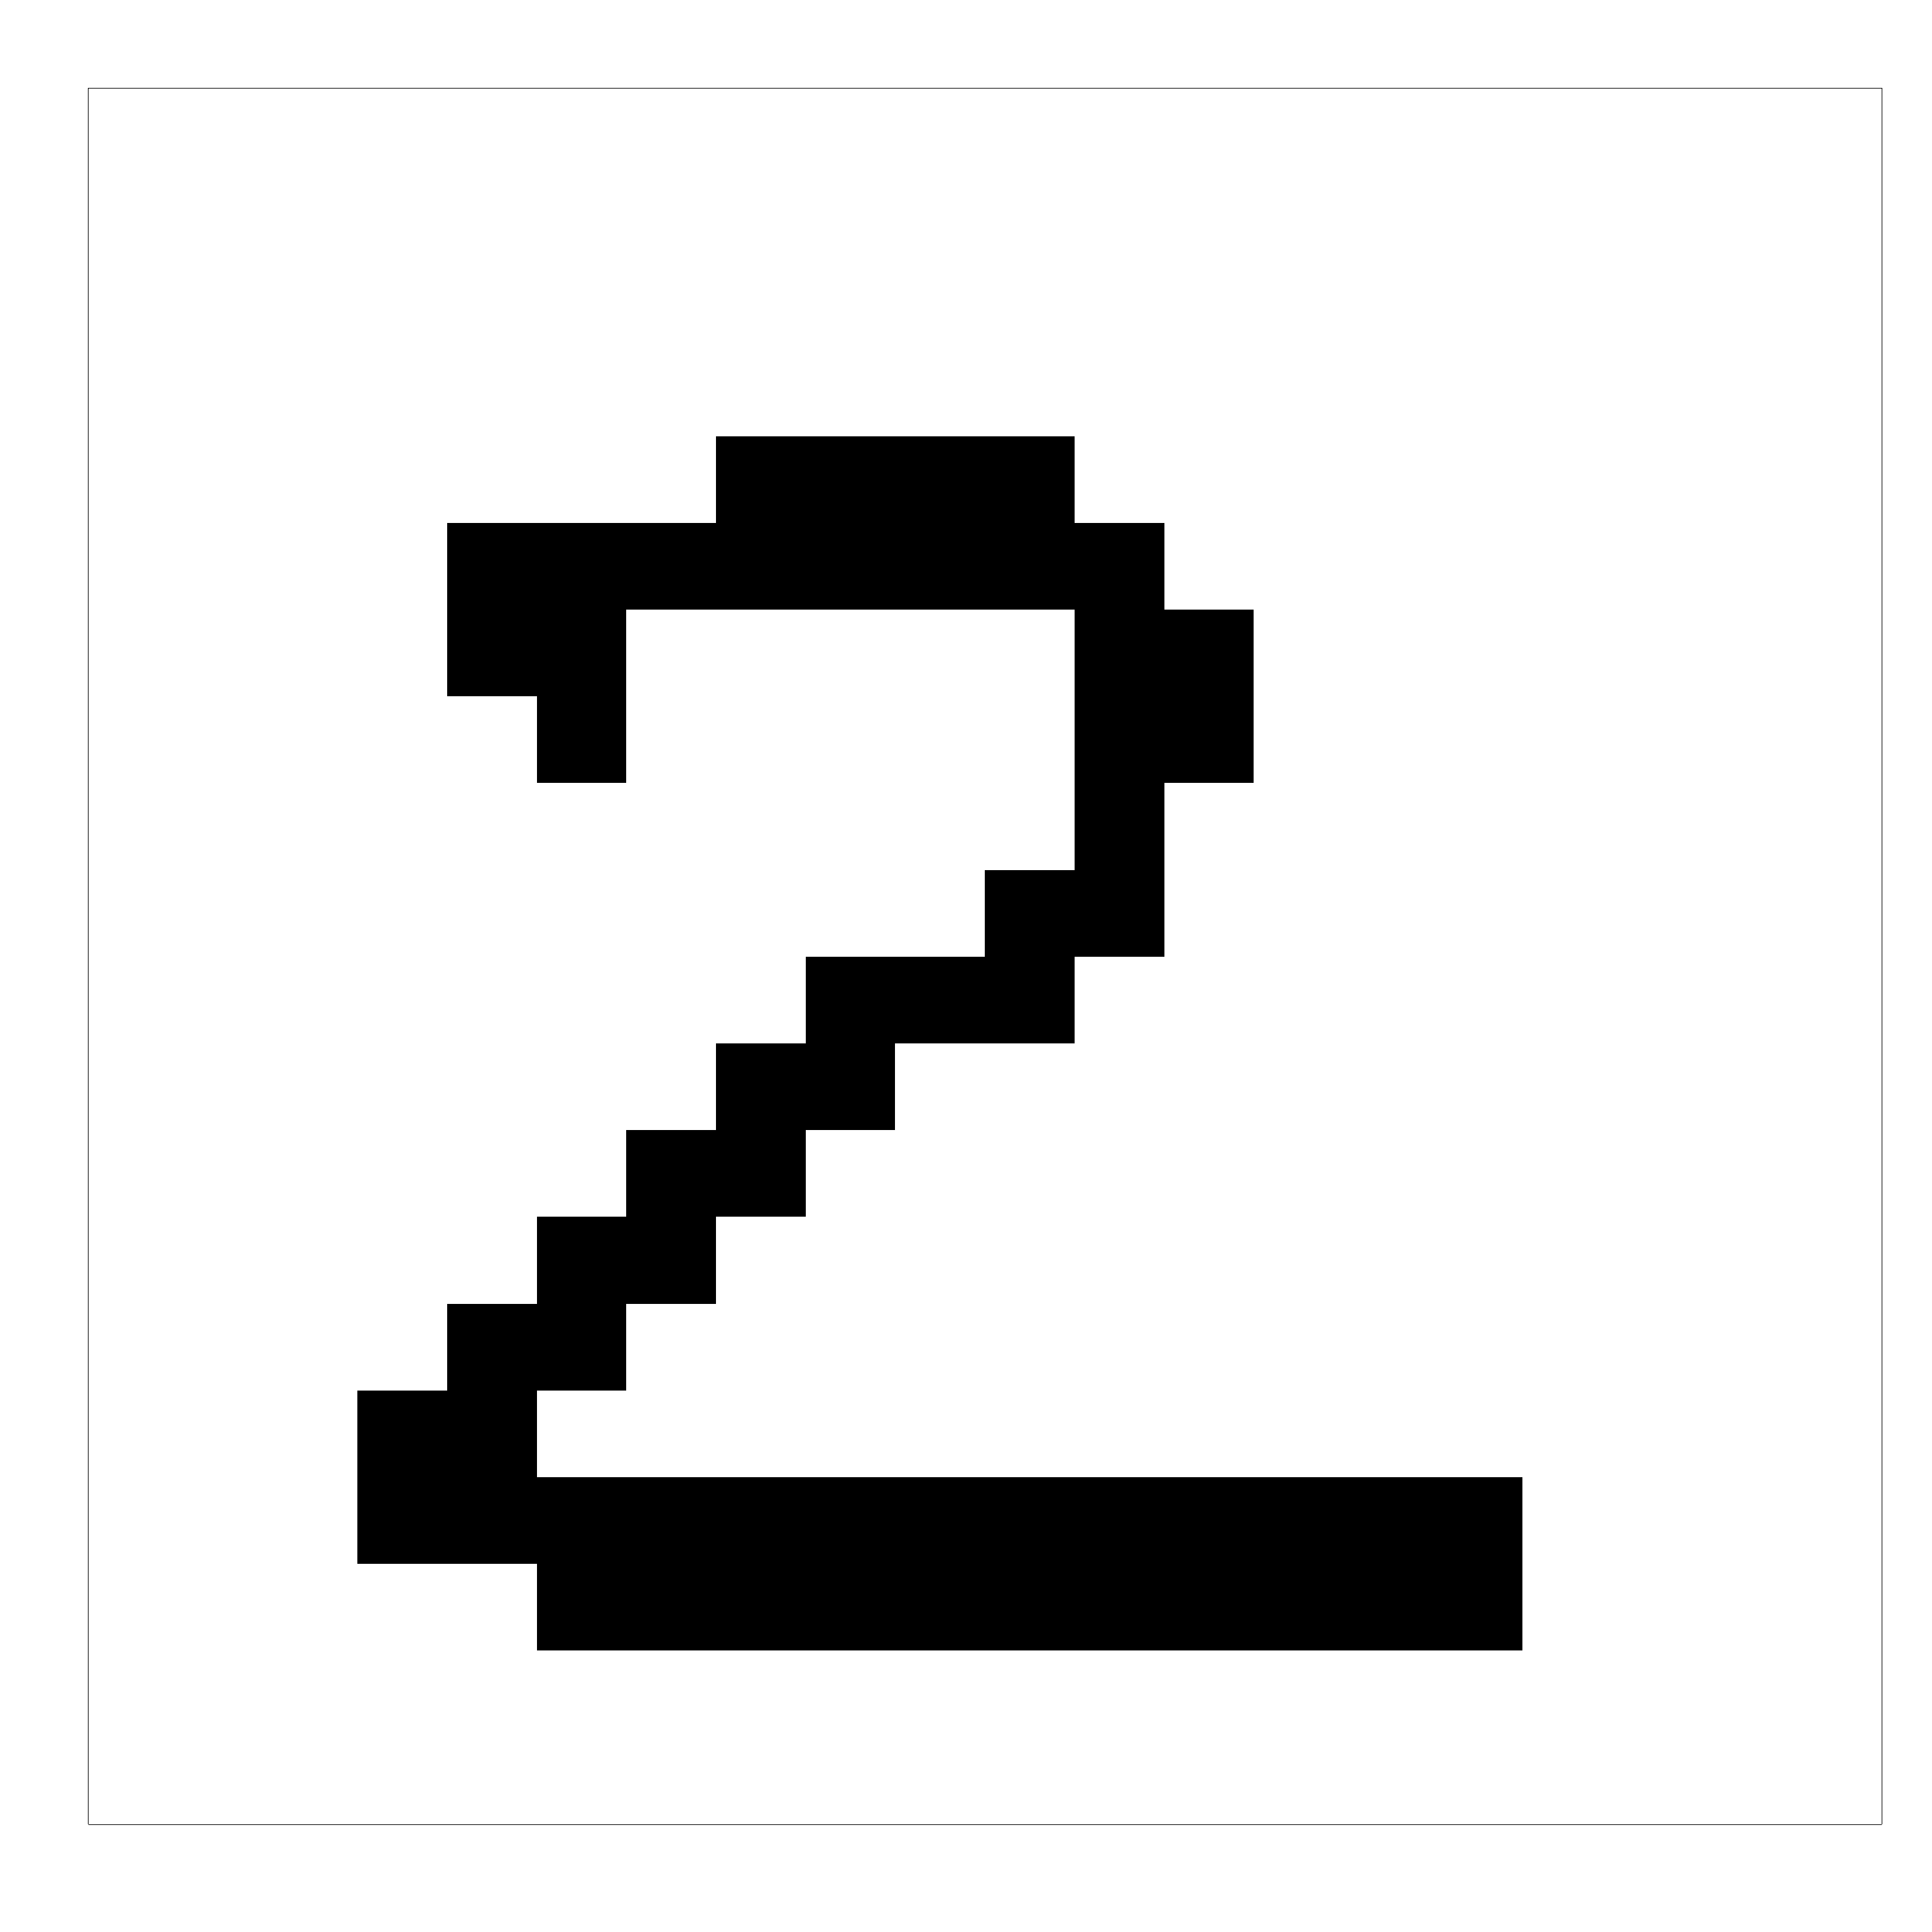
\includegraphics[width = \textwidth]{graphics/bins_2}
    \end{subfigure}
\caption{look at these beautiful 2's}
\end{figure}

\subsection{K-means}
K-means is used to group the data set into categories depending on their location in the x-dimensional space determined by the amount of features representing one of them.
The center of these clusters are then computed and identified as a specific category.
Using these centres, a unknown element can then be categorized depending on which cluster is the closest.

To find the number of clusters best representing the data set, then the within-group heterogeneity and homogeneity was computed for various K's as seen on figure \ref{fig:elbow_point}.
The elbow point can from here be determined to be at K of 1300 where it has 73.6\% homogeneity.

% It is also shown that normalizing the data or using a filter doesn't improve the performance. It actually hurts the performance. 

% k_means_elbow.R
\begin{figure}[H]
\centering
\begin{subfigure}{0.70\textwidth}
\centering
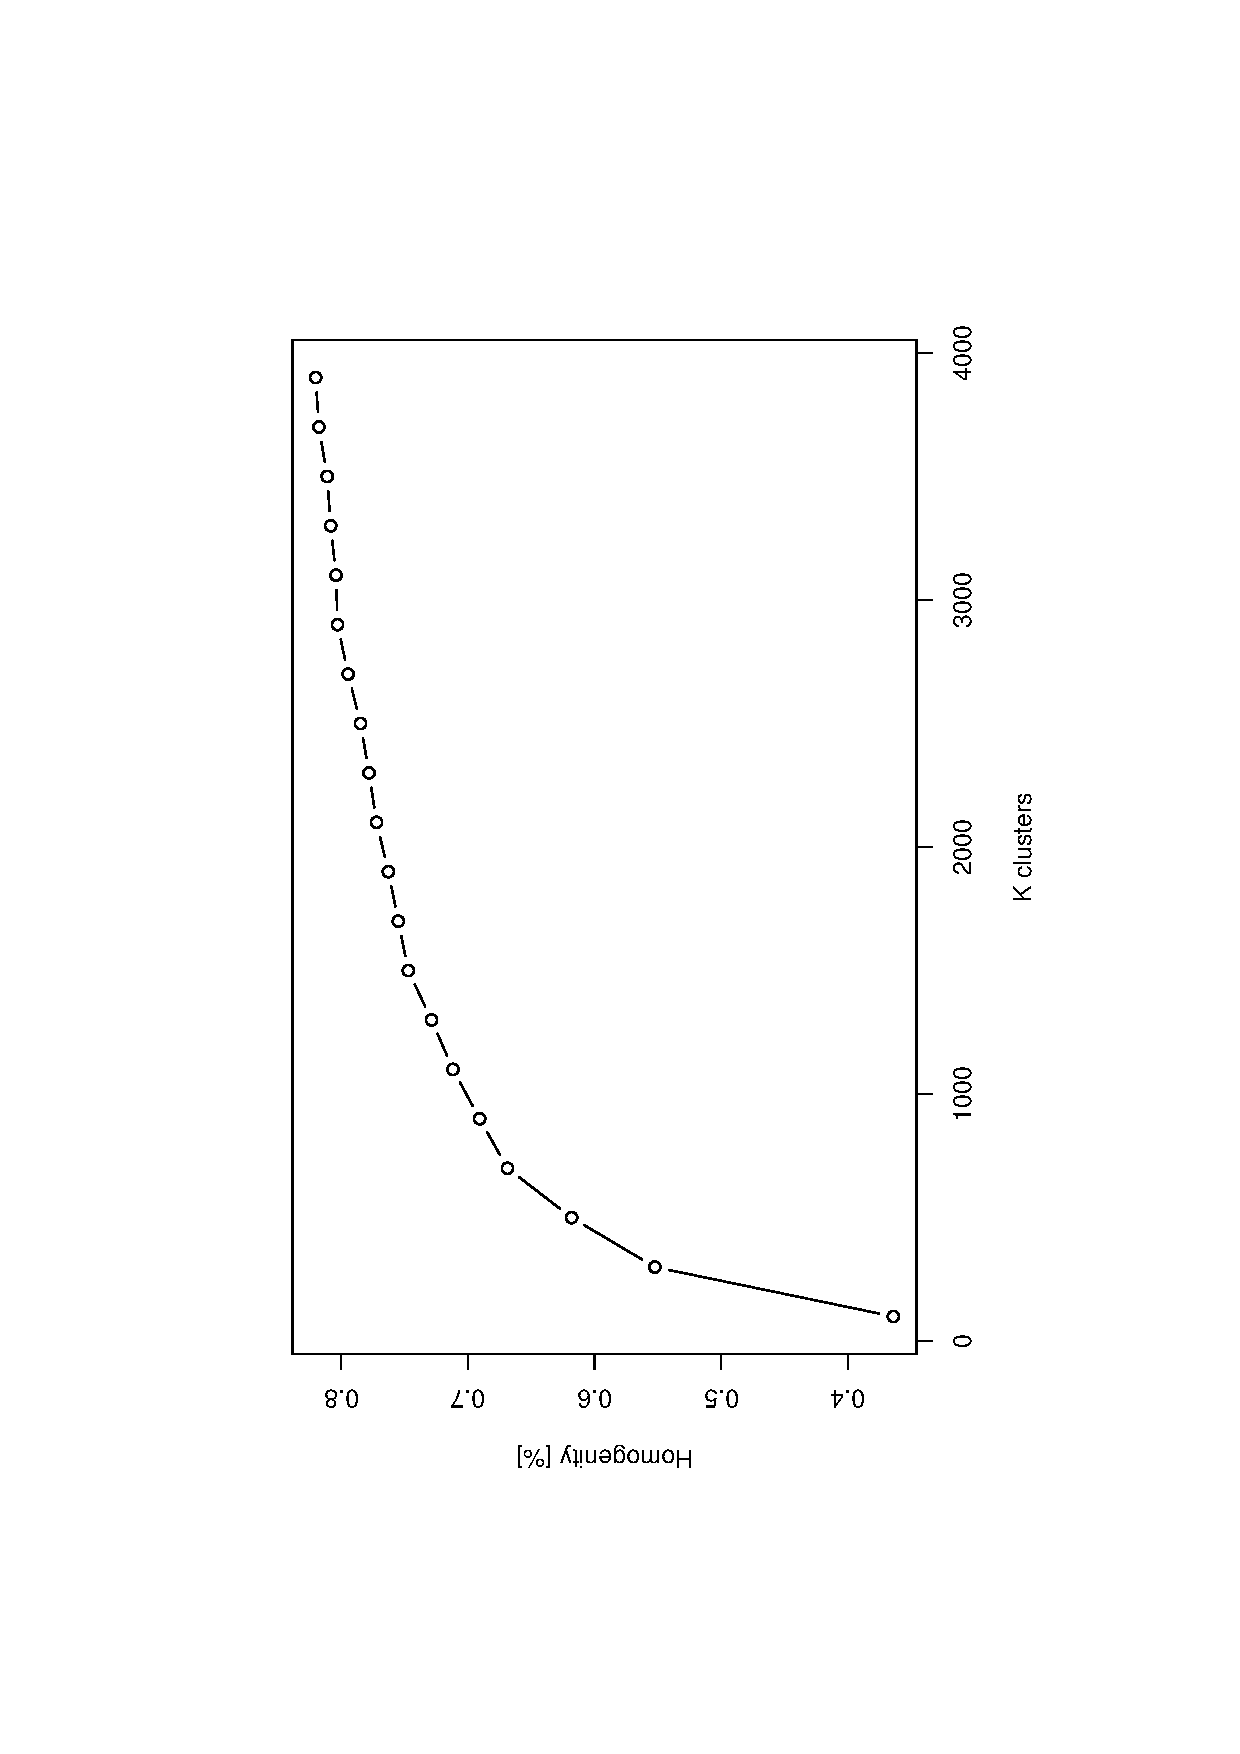
\includegraphics[width=\textwidth]{graphics/homogenity}
\caption{homogeneity}
\label{fig:homogeneity_kmean}
\end{subfigure}\\[-1cm]
\begin{subfigure}{0.70\textwidth}
\centering
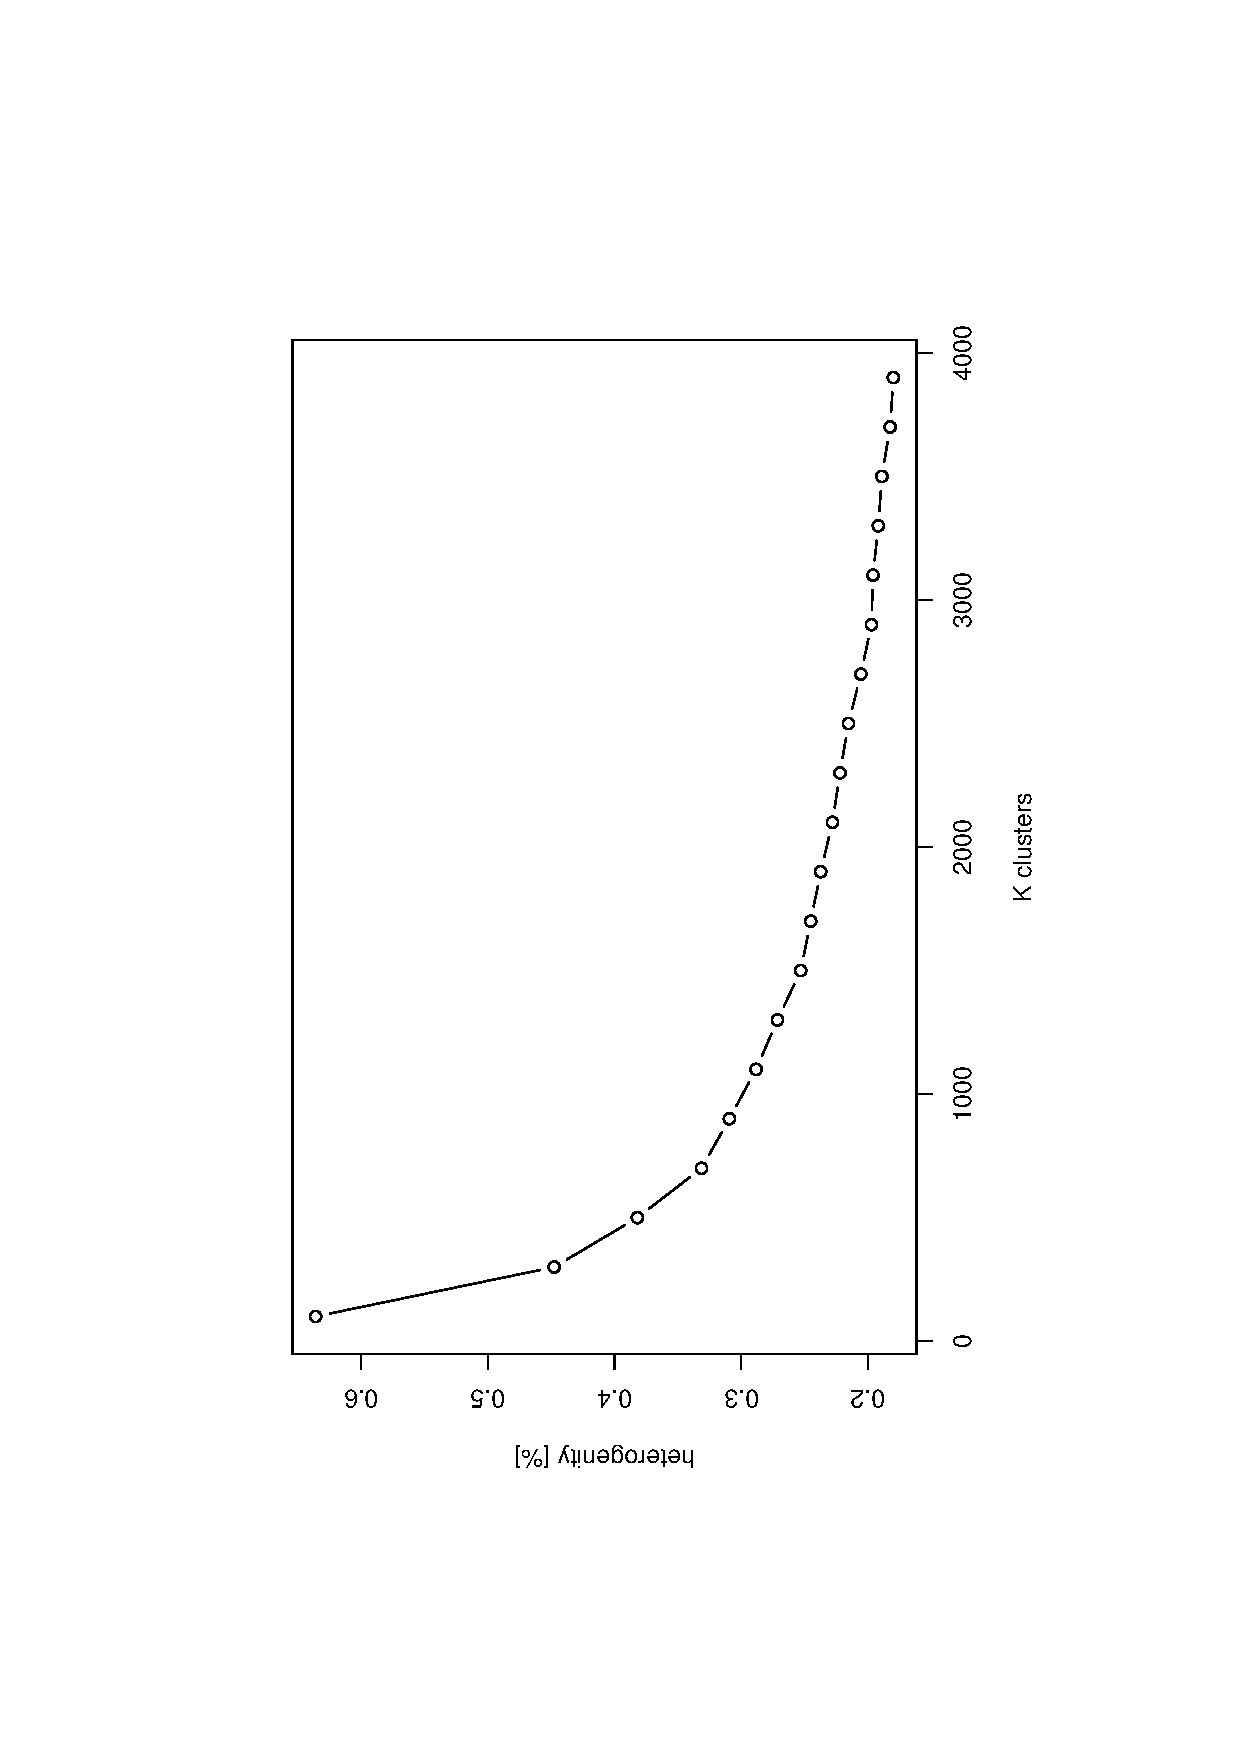
\includegraphics[width=\textwidth]{graphics/heterogenity}
\caption{heterogeneity}
\label{fig:heterogeneity_kmean}
\end{subfigure}
\caption[K means elbow point]{homogeneity and heterogeneity of the data set.}
\label{fig:elbow_point}
\end{figure}


\begin{table}[H]
\centering
%# kmean = 1500
%# k_knn = 10
%# k_mean = 10     
%# kmean_iterations = 500
%# Time taken to prep kmean: 747.229999999996
%# Time taken to run kmean classification: 42.1600000000035
%# Success for kmean: 0.54275
%# Time taken to prep norm kmean: 802.549999999996
%# Time taken to run norm kmean classification: 44.4400000000023
%# Success for norm kmean: 0.63125
%# Time taken to run raw knn classification: 1878.1
%# Success for raw knn: 0.73625

\begin{tabular}{|l|p{2cm}|p{2cm}|p{2cm}|}\hline
Criteria              & None   & K-mean & Normalized K-mean \\ \hline
Pre-Processing Time*  & 0s     & 12m27s & 13m23s            \\ \hline
Classification Time** & 31m18s & 42.2s  & 44.4s             \\ \hline
Success Rate**        & 73.6\% & 54.3\% & 63.1\%            \\ \hline
\multicolumn{4}{|l|}{* of 60,000 elements} \\ 
\multicolumn{4}{|l|}{** of 4,000 elements} \\ \hline
\end{tabular}

% \begin{tabular}{|l|p{2cm}|p{2cm}|p{2cm}|}\hline
% Criteria              & None    & K-mean  & Normalized K-mean  \\ \hline
% Pre-Processing Time*  & 0s      & 14m3.3s & 15m7.7s            \\ \hline
% Classification Time** & 18m1.7s & 43.5s   & 39.6s              \\ \hline
% Success Rate**        & 73.7\%  & 54.1\%  & 60.4\%             \\ \hline
% \multicolumn{4}{|l|}{* of 60,000 elements} \\ 
% \multicolumn{4}{|l|}{** of 4,000 elements against the training set.} \\ \hline
% \end{tabular}
\caption{Processing time comparison of running K-NN on K-mean data, normalized + k-mean data and raw data. 
K-mean makes 1300 clusters and max 500 iterations, the K-NN algorithm is applied with k = 10.}
\label{tab:processingtime_kmean_vs_raw_knn}
\end{table}

As seen in table \ref{tab:processingtime_kmean_vs_raw_knn} K-means clustering reduces the processing time at the cost of performance. 
Depending on the data set and the hardware this should be taken into consideration. 
Because K-means is a random algorithm the timing is unpredictable. If the starting points are very good the timing will decrease. 
A way to force this behaviour is to set a max iteration that is low enough so the timing will always be low.
This will cause the random selection to affect the performance. 
If a high enough max iteration is selected the timing might be so bad that K-means clustering is not worth the reduction in successful classifications.



\end{document}